\documentclass[11pt,a4paper]{article}
\usepackage[T1]{fontenc}
\usepackage[utf8]{inputenc}
\usepackage{lmodern}
\usepackage[margin=2.5cm]{geometry}
\usepackage{amsmath,amssymb}
\usepackage{booktabs}
\usepackage{graphicx}
\usepackage{float}
\usepackage{caption}
\usepackage{enumitem}
\usepackage{microtype}
\usepackage{xcolor}
\usepackage[round]{natbib}
\usepackage[colorlinks=true,linkcolor=blue!50!black,urlcolor=blue!50!black,citecolor=blue!50!black]{hyperref}

\setlist{itemsep=2pt,topsep=4pt}
\emergencystretch=3em
\captionsetup{font=small,labelfont=bf}

\newcommand{\iu}{\mathrm{i}}
\newcommand{\code}[1]{\texttt{#1}}
\DeclareMathOperator{\Arg}{Arg}
\DeclareMathOperator{\wrap}{wrap}
\DeclareMathOperator{\E}{E}
\DeclareMathOperator{\RMSE}{RMSE}
\newcommand{\1}{\mathbf{1}}
\renewcommand{\Re}{\operatorname{Re}}
\renewcommand{\Im}{\operatorname{Im}}


\title{Point and probabilistic forecasts of wind with complex ARIMA:\\ design and results of the second experiment}
\author{Wind Forecasting with Complex ARIMA --- working notes}
\date{26 October 2026}

\begin{document}
\maketitle

\section{Purpose}

The paper models wind as a single complex variable, combining speed and direction, with complex
ARIMA (cARIMA). The first experiment (note of 30 September 2026) compared the point forecasts of
cARIMA with persistence and with pairs of real ARIMA models, up to 6 hours ahead. This note
describes the second experiment, which responds to the comments on that note:
\begin{enumerate}
  \item \textbf{The cAR(0) models looked strange} (most models chosen on the selection window had
    no AR term). The orders are now chosen by cross-validation on separate forecast origins, and
    the accuracy of every order is reported on the test origins (Sections~\ref{sec:selection}
    and~\ref{sec:orders}).
  \item \textbf{Horizon up to 2 hours}: $h = 1, \dots, 12$ steps of 10 minutes, for the choice of
    the orders, the forecasts and the evaluation.
  \item \textbf{Phase plane}: magnitude against angle for $Z_t$ and $\log Z_t$, and for their
    changes $\Delta Z_t$ and $\Delta\log Z_t$ (Section~\ref{sec:phase}).
  \item \textbf{cARIMA in logarithms with a real constant}: a drift in log speed but none in
    the direction (Section~\ref{sec:constant}).
  \item \textbf{Predictive distributions}: the quantiles $\tau = 0.01, 0.02, \dots, 0.99$ of
    speed and direction for every model, evaluated by the pinball score for each quantile and by
    calibration plots (Sections~\ref{sec:distributions} and~\ref{sec:probabilistic}).
\end{enumerate}
The data and the models are the same as in the first experiment; Sections~\ref{sec:data}
and~\ref{sec:models} repeat their description so that this note can be read on its own.

\section{Data}\label{sec:data}

\begin{itemize}
  \item \textbf{Source.} The Kaggle ``Wind Turbine SCADA'' dataset, file \code{T1.csv}. SCADA
    (supervisory control and data acquisition) is the monitoring system of a wind turbine; it
    records measurements at the turbine, here every 10 minutes. The file covers one turbine in
    Turkey for the whole of 2018 and contains wind speed (m/s) and wind direction (degrees).
    More details are in \code{data/README.md}.
  \item \textbf{Missing values.} A complete 10-minute grid for 2018 has 52,560 time points; the
    file has 50,530 of them. The 2,030 missing points include three gaps longer than 3 days.
  \item \textbf{Preparation} (\code{R/02\_prepare\_data.R}):
  \begin{itemize}
    \item the data are put on the complete 10-minute grid, with the missing points left empty;
    \item gaps of at most 36 points (6 hours) are filled by linear interpolation of the two
      Cartesian coordinates of the wind vector, $\Re Z_t$ and $\Im Z_t$ (defined in
      Section~\ref{sec:complex});
    \item the 10 zero speeds are replaced by 0.1\,m/s, so that the logarithm of speed exists.
  \end{itemize}
\end{itemize}

The 10-minute changes of wind are heavy-tailed: most changes are small, but some are very large.
Table~\ref{tab:kurt} gives the kurtosis $\E(x - \E x)^4/(\operatorname{Var} x)^2$ of the changes
between consecutive observations. It equals 3 for a normal distribution; larger values mean
heavier tails. All four changes are far from normal. About 3\% of the direction changes exceed
$30^\circ$, and 0.5\% exceed $90^\circ$. The changes of the Cartesian coordinates combine changes of speed and of direction, and
$\Re Z_t$ has the heaviest tails of all: a sudden turn at high speed moves the wind vector a long way.

Figure~\ref{fig:hist} shows the same changes as histograms with the counts on a log scale, so that
the tails are visible; a normal distribution would appear as a parabola.
\begin{itemize}
  \item \textbf{Left, change of log speed.} The distribution is sharply peaked at zero: half of the
    changes are within $\pm 0.06$ (about $\pm 6\%$ of the speed), with a standard deviation of
    0.16. But the counts decay roughly linearly on the log scale, i.e.\ exponentially rather than
    like a normal distribution, and reach changes of $-1.6$ and $+2.4$ (speeds falling to a fifth or
    rising elevenfold within 10 minutes). Such large relative changes happen at low speeds: in all 66
changes larger than 1 in absolute value, one of the two speeds is below 3.7\,m/s.
  \item \textbf{Middle, change of the recorded angle.} Besides the central peak there are two side
    peaks near $\pm 2\pi$. They are not real turns of the wind but the artificial jumps that occur
    when the direction crosses $\pm\pi$ (696 times; Section~\ref{sec:diff}). Because of them the
    standard deviation is 0.71\,rad.
  \item \textbf{Right, shortest-arc change of direction.} With the jumps removed, the side peaks
    disappear and the standard deviation falls to 0.25\,rad ($14^\circ$). The centre is again very
    narrow (half of the changes are within about $\pm 3^\circ$), and the tails are heavy and extend
    to $\pm\pi$: there are 63 turns of more than $150^\circ$ within 10 minutes.
\end{itemize}
These heavy tails motivate the heavy-tailed error distribution in
Section~\ref{sec:cgnorm}, and the side peaks motivate the unwrapping of the angle in
Section~\ref{sec:diff}.

\begin{table}[H]
  \centering
  \caption{Kurtosis of the changes between consecutive 10-minute observations (normal
    distribution: 3). $v_t$ is speed, $\theta_t$ direction and $Z_t$ the wind as a complex number
    (Section~\ref{sec:complex}); $\wrap(\cdot)$ is defined in \eqref{eq:unwrap}.}\label{tab:kurt}
  \begin{tabular}{lr}
    \toprule
    change & kurtosis \\
    \midrule
    $\log v_t - \log v_{t-1}$ & 14.4 \\
    $\wrap(\theta_t - \theta_{t-1})$ & 52.8 \\
    $\Re Z_t - \Re Z_{t-1}$ & 131.9 \\
    $\Im Z_t - \Im Z_{t-1}$ & 25.5 \\
    \bottomrule
  \end{tabular}
\end{table}

\begin{figure}[H]
  \centering
  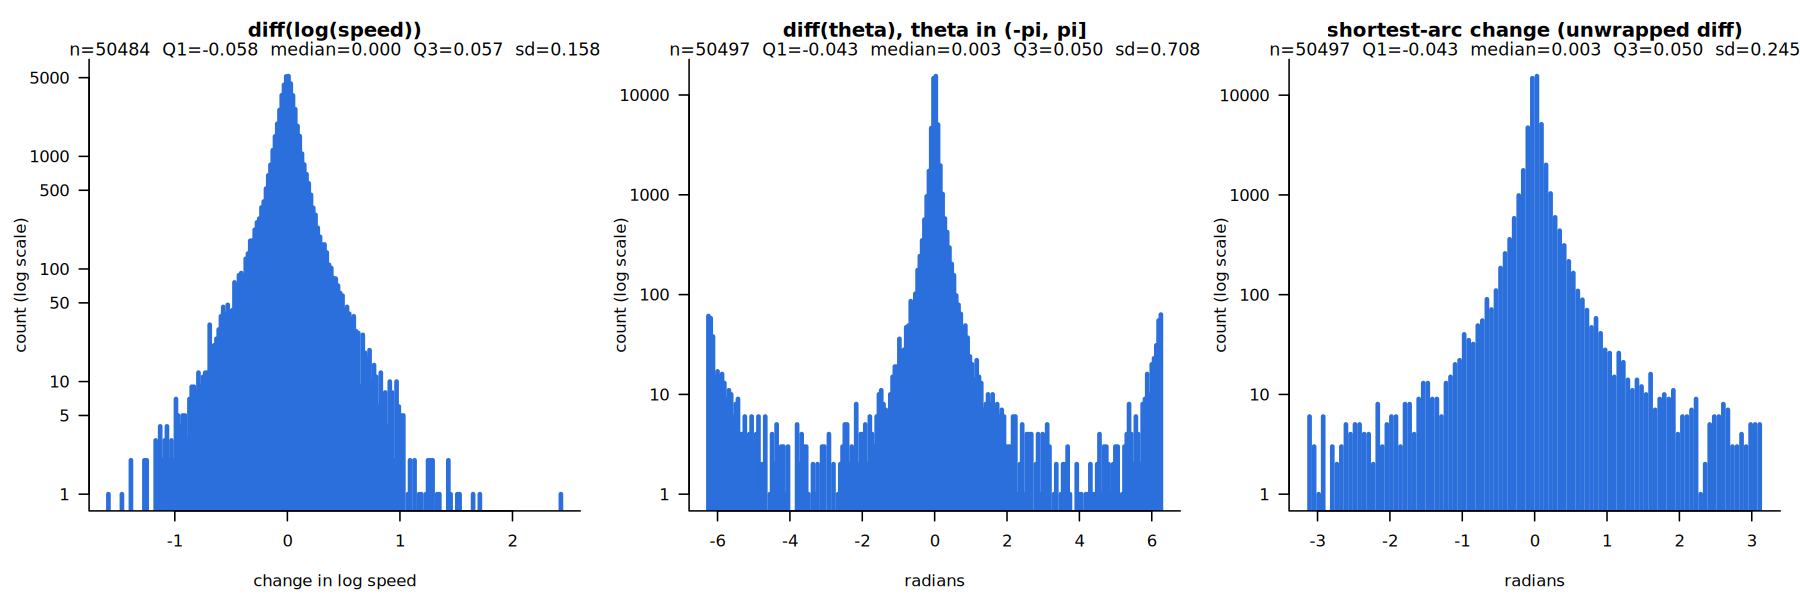
\includegraphics[width=\textwidth]{../figures/diffs_hist.png}
  \caption{Histograms of the changes between consecutive 10-minute observations, counts on a log
    scale. Left: change of log speed. Middle: change of the direction angle as recorded in
    $(-\pi, \pi]$, in radians. Right: shortest-arc change of direction, in radians. The line above
    each panel gives the number of changes, the quartiles and the standard deviation.}\label{fig:hist}
\end{figure}

\subsection{Phase plane}\label{sec:phase}

Figures~\ref{fig:phase} and~\ref{fig:phase-diff} plot the magnitude (horizontal axis) against
the angle (vertical axis) for all 10-minute observations of 2018 (\code{R/08\_phase\_plane.R}). In
Figure~\ref{fig:phase} the angle of $\log Z_t$ uses the recorded direction in $(-\pi, \pi]$.
\begin{itemize}
  \item \textbf{$Z_t$ (Figure~\ref{fig:phase}, left).} Speed against direction. The two
    prevailing directions, about $60^\circ$ and $-160^\circ$ to $180^\circ$, are horizontal bands,
    and the strongest winds come from them. Other directions occur mostly at low speeds.
  \item \textbf{$\log Z_t$ (right).} $|\log Z_t| = \sqrt{\log^2 v_t + \theta_t^2}$ against
    $\Arg\log Z_t = \operatorname{atan2}(\theta_t, \log v_t)$. The two prevailing directions become
    two tight bands, at about $+25^\circ$ and $-50^\circ$, which narrow as the speed grows.
  \item \textbf{$\Delta Z_t = Z_t - Z_{t-1}$ (Figure~\ref{fig:phase-diff}, left).} The 10-minute
    changes of the wind vector go in all directions with no preferred angle; half of them are
    shorter than 0.62\,m/s.
  \item \textbf{$\Delta\log Z_t = \log(v_t/v_{t-1}) + \iu\wrap(\theta_t - \theta_{t-1})$ (right).}
    The changes the models with $d = 1$ work on. They concentrate near the angles $0^\circ$ and
    $\pm 180^\circ$: most 10-minute changes are mainly a change of log speed, with a much smaller
    change of direction (in radians). The large changes, to the right, are spread over all angles.
\end{itemize}
Differences are only taken between consecutive observed points (50,707 pairs), and the horizontal
axes of Figure~\ref{fig:phase-diff} are cut at the 99.5\% quantile of the modulus (the maxima are
34\,m/s and 5.6).

\begin{figure}[H]
  \centering
  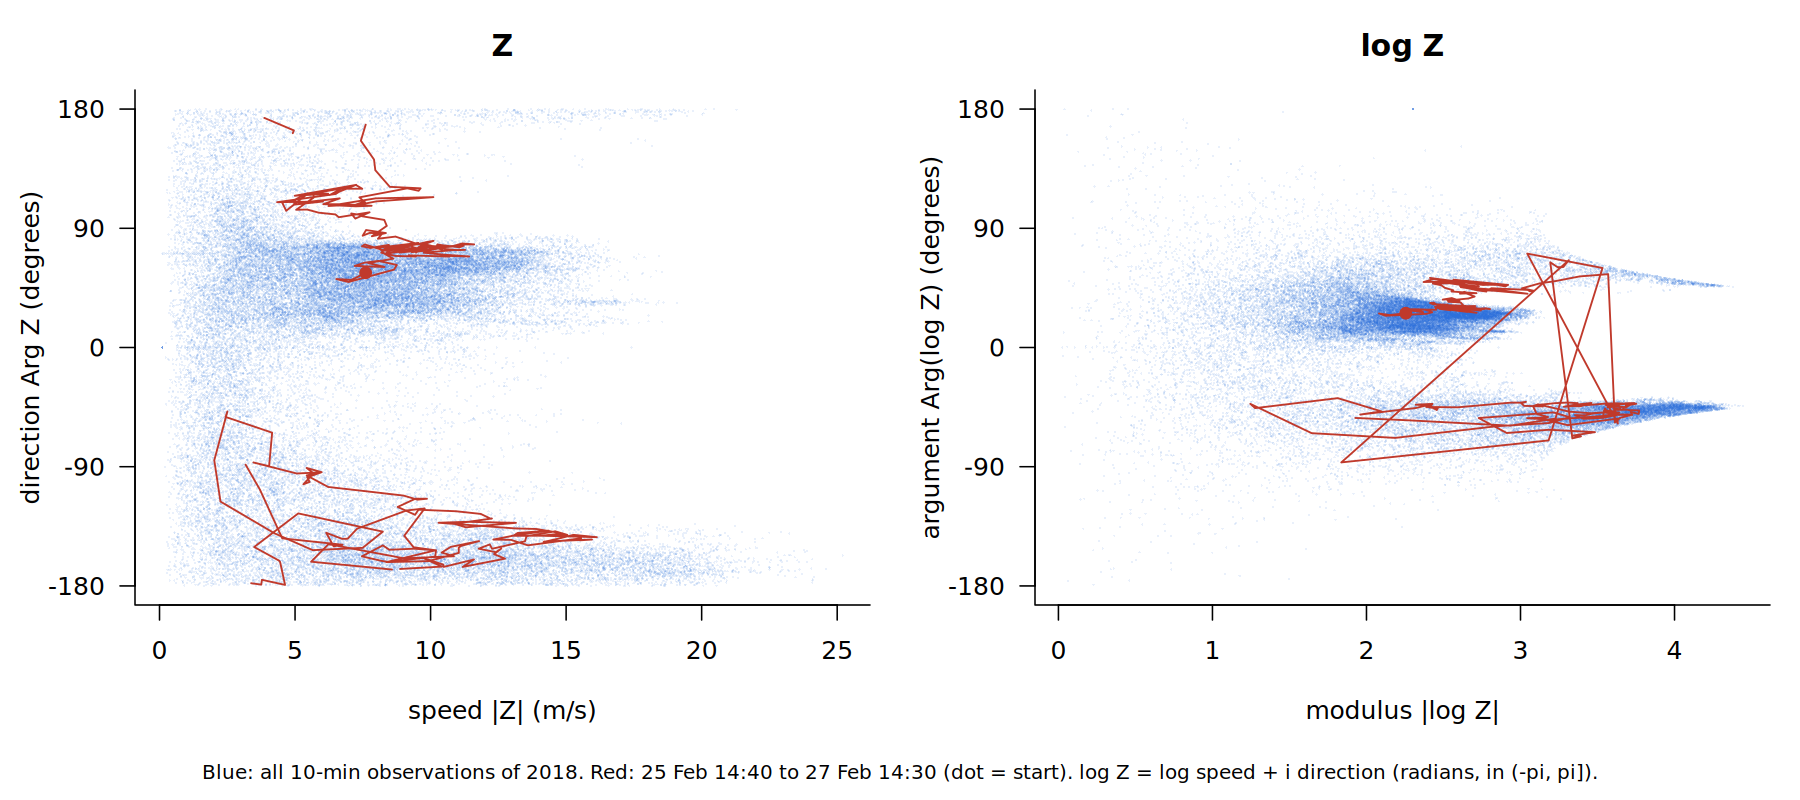
\includegraphics[width=\textwidth]{../figures/phase_plane.png}
  \caption{Phase plane of $Z_t$ (speed against direction) and of $\log Z_t$ (modulus against
    argument), all 10-minute observations of 2018.}\label{fig:phase}
\end{figure}

\begin{figure}[H]
  \centering
  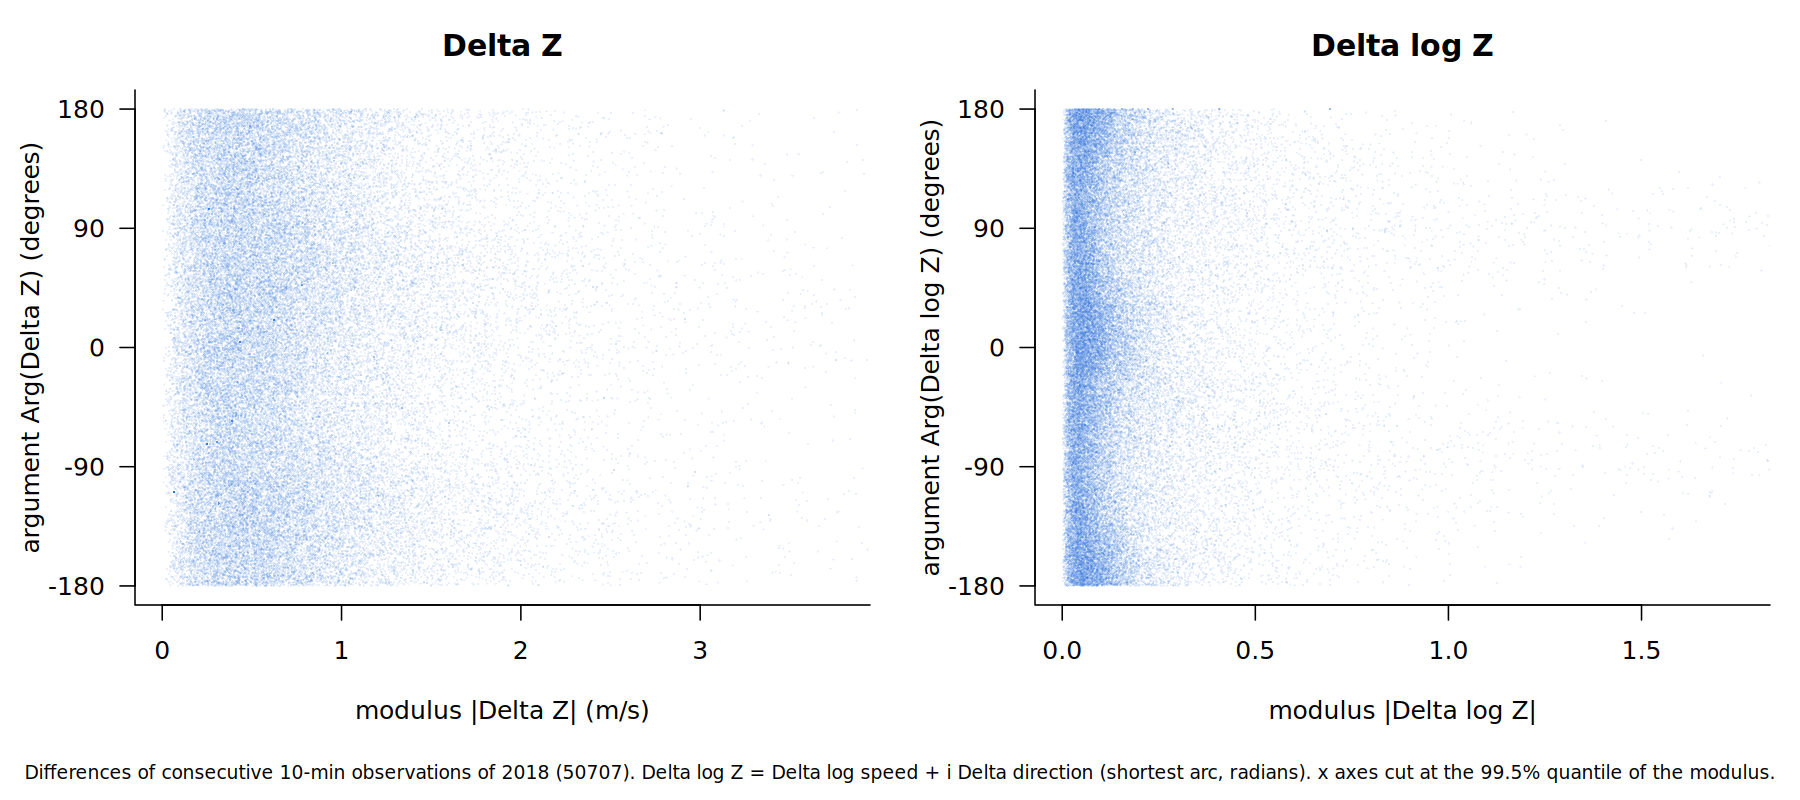
\includegraphics[width=\textwidth]{../figures/phase_plane_diff.png}
  \caption{Phase plane of the 10-minute changes $\Delta Z_t$ and $\Delta\log Z_t$ (modulus against
    argument).}\label{fig:phase-diff}
\end{figure}

\section{How the wind is modelled}\label{sec:models}

\subsection{Wind as a complex number}\label{sec:complex}

With speed $v_t > 0$ and direction angle $\theta_t \in (-\pi, \pi]$ (in radians), the wind at time
$t$ is
\begin{equation}
  Z_t = v_t e^{\iu\theta_t} = v_t\cos\theta_t + \iu\, v_t\sin\theta_t .
\end{equation}
The modulus $|Z_t|$ is the speed and the argument $\Arg Z_t$ is the direction. $\Re Z_t$ and
$\Im Z_t$ are the Cartesian coordinates of the wind vector. They are not the zonal and meridional
components used in meteorology, which are measured along the east and north axes; here the angle
is simply the recorded direction.

\subsection{Complex ARIMA}

The cARIMA$(p,d,q)$ model for a complex series $y_t$ is
\begin{equation}\label{eq:carima}
  \Bigl(1 - \sum_{j=1}^{p}\phi_j B^j\Bigr)(1-B)^d\, y_t
  = \beta_0 + \Bigl(1 + \sum_{j=1}^{q}\theta_j B^j\Bigr)\varepsilon_t,
  \qquad \phi_j, \theta_j, \beta_0 \in \mathbb{C},
\end{equation}
where $B$ is the backshift operator ($B y_t = y_{t-1}$), $p$ and $q$ are the autoregressive (AR) and
moving average (MA) orders, and $d$ is the order of differencing. With $d = 1$ the constant
$\beta_0$ is a \emph{drift}: a fixed complex change added at every step. With $d = 0$ it
determines the mean of the series, $\beta_0 / (1 - \sum_j \phi_j)$.

Multiplying by a complex coefficient $\phi = a + \iu b = r e^{\iu\alpha}$ \emph{scales} by
$r = |\phi|$ and \emph{rotates} by $\alpha = \Arg\phi$. For the pair $(\Re y, \Im y)$,
\begin{equation}
  \begin{pmatrix} \Re(\phi y) \\ \Im(\phi y) \end{pmatrix}
  = \begin{pmatrix} a & -b \\ b & a \end{pmatrix}
    \begin{pmatrix} \Re y \\ \Im y \end{pmatrix},
\end{equation}
so cARIMA is a bivariate VARIMA whose coefficient matrices are restricted to this form: 2 real
parameters per lag instead of 4.

The models are estimated by maximum likelihood with \code{complex::clm()}. It fits
\eqref{eq:carima} for the series in levels: the observations lost to differencing and lags at the
start of the sample are filled in by extrapolation, and the forecasts are produced directly for
$y_t$ rather than for its differences.

\subsection{The error distribution and non-circularity}\label{sec:error}

In the basic model, the error $\varepsilon_t$ is \emph{complex normal}. For a complex random
variable with zero mean, two second moments are needed, and we use the terms of
\citet{svetunkov2024}:
\begin{itemize}
  \item the \emph{conjugate variance} $\sigma^2 = \E(\varepsilon_t\bar\varepsilon_t) =
    \E|\varepsilon_t|^2$, computed with the complex conjugate; it is real and measures the overall
    size of the error;
  \item the \emph{direct variance} $\varsigma^2 = \E(\varepsilon_t^2)$, computed without the
    conjugate (elsewhere called the pseudo-variance); it is complex in general and describes the
    shape of the error cloud in the plane.
\end{itemize}
Together they give the covariance matrix of the real and imaginary parts:
\begin{equation}
  \operatorname{Var}(\Re\varepsilon_t) = \tfrac12(\sigma^2 + \Re\varsigma^2), \quad
  \operatorname{Var}(\Im\varepsilon_t) = \tfrac12(\sigma^2 - \Re\varsigma^2), \quad
  \operatorname{Cov}(\Re\varepsilon_t, \Im\varepsilon_t) = \tfrac12\Im\varsigma^2 .
\end{equation}
With $\varsigma^2 = 0$ the error is \emph{circular}: the two parts have the same variance and are
uncorrelated, so the cloud of errors is a circle. With $\varsigma^2 \neq 0$ it is
\emph{non-circular}: the cloud is an ellipse. For wind, non-circularity means that the changes of
the wind vector are larger along some directions than others. We measure it by the ratio of the
two variances,
\begin{equation}\label{eq:noncirc}
  \kappa = \frac{|\varsigma^2|}{\sigma^2} \in [0, 1],
\end{equation}
which is 0 for a circular error and 1 for an error that always lies on one line. A pair of
independent real models, one for $\Re Z_t$ and one for $\Im Z_t$, ignores the correlation between
the two errors.

\subsection{The complex generalised normal distribution}\label{sec:cgnorm}

Because the changes of wind are heavy-tailed (Table~\ref{tab:kurt}), the models are also
estimated with a \emph{complex generalised normal} error (\citealp{novey2010};
\code{distribution = "dcgnorm"} in \code{clm()}). For the error $e = z - \mu$, with conjugate
scale $\alpha^2 > 0$, direct scale $\psi^2 \in \mathbb{C}$ ($|\psi^2| < \alpha^2$) and shape
$\beta > 0$, the density is
\begin{equation}\label{eq:cgnorm}
  f(z) = \frac{2\beta}{\pi\,\Gamma(1/\beta)\, 2^{1/\beta}\sqrt{\alpha^4 - |\psi^2|^2}}
         \exp\Bigl(-\tfrac12 Q^\beta\Bigr),
  \qquad
  Q = \frac{2\bigl(\alpha^2|e|^2 - \Re(\overline{\psi^2}\, e^2)\bigr)}{\alpha^4 - |\psi^2|^2}.
\end{equation}
\begin{itemize}
  \item $\beta = 1$ gives the complex normal distribution with conjugate variance $\alpha^2$ and
    direct variance $\psi^2$. A shape $\beta < 1$ gives heavier tails ($\beta = 0.5$ is similar to
    the Laplace distribution); $\beta > 1$ gives lighter tails.
  \item For other $\beta$, the conjugate and direct variances equal $\alpha^2$ and $\psi^2$
    multiplied by $2^{1/\beta}\Gamma(2/\beta) / (2\Gamma(1/\beta))$. In \code{dcgnorm()} the two scales
    are the arguments \code{scaleConjugate} and \code{scaleDirect}.
  \item The shape $\beta$ is estimated together with the ARIMA coefficients. For any given values
    of these, the maximum likelihood estimates of the two scales have a closed form, so
    they are substituted into the likelihood (``concentrated out'') and not searched for
    numerically.
\end{itemize}
With heavy tails, a few very large changes can pull the estimates of a normal model, in
particular the drift. A heavy-tailed likelihood gives these observations less weight.

\subsection{Why logarithms}\label{sec:log}

Besides $Z_t$ itself, the models are applied to the complex logarithm of the wind,
\begin{equation}
  \log Z_t = \log v_t + \iu\,\tilde\theta_t ,
\end{equation}
where $\tilde\theta_t$ is the unwrapped direction angle (Section~\ref{sec:diff}).
\begin{itemize}
  \item The logarithm \emph{separates speed and direction}: the real part is log speed and the
    imaginary part is the angle. A cARIMA for $\log Z_t$ is still one complex model: the two parts
    are linked through the complex coefficients and the error covariance.
  \item Changes of speed are roughly \emph{proportional} to the speed (larger when it is windy), so
    log speed is a more natural scale than speed.
  \item Forecasts are transformed back by $\hat Z = \exp(\widehat{\log Z})$, which always gives a
    positive speed and a valid direction.
  \item $\exp(\widehat{\log Z})$ is not the expected value of $Z$; no correction for this is made.
  \item The drift of a model for $\log Z_t$ with $d = 1$ has a direct meaning: $\Re\beta_0$ is a
    steady percentage change of speed, and $\Im\beta_0$ is a steady rotation of the direction, in
    radians per 10 minutes. There is no physical reason for the wind to keep turning in one
    direction for weeks, so models for $\log Z_t$ are also fitted without the constant, and with
    the real part of the constant only (Section~\ref{sec:constant}).
\end{itemize}

\subsection{Differences and unwrapping of the angle}\label{sec:diff}

\begin{itemize}
  \item At 10-minute resolution the wind is very persistent: over several weeks its level wanders
    without returning to a stable mean. The models are therefore fitted mainly to changes,
    $d = 1$. In logarithms the differences have a clear meaning:
    \begin{equation}
      (1-B)\log Z_t = \log\frac{v_t}{v_{t-1}} + \iu\,(\tilde\theta_t - \tilde\theta_{t-1}),
    \end{equation}
    the log ratio of consecutive speeds plus $\iu$ times the change of direction.
  \item The recorded angle jumps by about $2\pi$ whenever the direction crosses $\pm\pi$. For
    example, a turn from $179^\circ$ to $-179^\circ$ is a change of $2^\circ$, but the recorded
    values differ by $358^\circ$. This happens 696 times in \code{T1.csv}. In differences these
    jumps would appear as huge artificial shocks (Figure~\ref{fig:hist}, middle).
  \item The angle is therefore \emph{unwrapped} within each estimation window $t = 1, \dots, T$:
    \begin{equation}\label{eq:unwrap}
      \tilde\theta_1 = \theta_1, \qquad
      \tilde\theta_t = \tilde\theta_{t-1} + \wrap(\theta_t - \theta_{t-1}), \qquad
      \wrap(x) = \operatorname{atan2}(\sin x, \cos x) \in (-\pi, \pi].
    \end{equation}
    $\wrap(\cdot)$ returns the equivalent angle in $(-\pi, \pi]$, so each step of $\tilde\theta_t$
    is the \emph{shortest-arc} change of direction, and $\tilde\theta_t$ can leave $(-\pi, \pi]$.
    Forecasts of the direction are wrapped back into $(-\pi, \pi]$ for evaluation.
  \item The unwrapped angle is used in $\log Z_t$ and in the real benchmark models for the
    angle (Section~\ref{sec:selection}). $Z_t$ itself needs no unwrapping: it is continuous when
    the direction crosses $\pm\pi$, because $\cos$ and $\sin$ are periodic.
  \item For $Z_t$, $d = 0$ is also a plausible choice: the wind vector could revert to a mean.
    One set of models chooses $d \in \{0, 1\}$ automatically (Section~\ref{sec:selection}).
\end{itemize}


\subsection{The constant}\label{sec:constant}

With the partial intercept of \code{clm()}, the constant $\beta_0$ of \eqref{eq:carima} can be
complex, real, imaginary or absent (in the formula: \code{y \textasciitilde{} 1},
\code{y \textasciitilde{} 1 - Im(1)}, \code{y \textasciitilde{} 1 - Re(1)},
\code{y \textasciitilde{} -1}). For $\log Z_t$ with $d = 1$, a real constant is a steady
percentage change of speed with no rotation of the direction. In the first experiment, the
complex constant of the normal model rotated the direction forecasts by about $0.7^\circ$ per 10
minutes and made them worse. Three constants are therefore compared for $\log Z_t$: complex, real
only (suffix \code{\_re}) and none (suffix \code{\_nd}).

\section{Design of the forecasting study}\label{sec:design}

\subsection{Rolling origin}

As in the first experiment, the models are repeatedly estimated on a window of past data and
forecast the next 2 hours, for many different ends of the window.
\begin{itemize}
  \item The estimation window is the 4 weeks up to the forecast origin ($T = 4032$
    observations), and the horizon is $h = 1, \dots, 12$ steps ahead (10 minutes to 2 hours).
  \item The \emph{test origins} are the same 300 origins as in the first experiment, from
    2018-02-27 14:40 to 2018-12-31 17:50 (all of them remain usable with the shorter horizon).
    The results are therefore directly comparable with the first 12 horizons of the first
    experiment; for persistence they are identical.
  \item At every origin, the parameters of all models are estimated again on that origin's
    window; only the orders stay fixed.
\end{itemize}

\subsection{Choice of model orders}\label{sec:selection}

\begin{itemize}
  \item \textbf{cARIMA with $d = 1$: cross-validation.} 100 \emph{cross-validation origins} are
    spread evenly over the usable origins from 2018-02-27 16:40 to 2018-12-31 21:50 (13--15 in each
    month from March to September except June, which has 1; 5 in November, 9 in December and 1 at
    the end of February). Each is at least 12
    steps away from every test origin, so no cross-validation forecast covers the same 2 hours as a
    test forecast; their estimation windows do overlap the test windows, as there is no earlier
    data. At every cross-validation origin, all 16 models with $p, q \in \{0, \dots, 3\}$ are
    estimated and forecast; the orders with the lowest RMSE of the wind vector over the 100
    origins and $h = 1, \dots, 12$ (Section~\ref{sec:measures}) are chosen, separately for each
    variant (series, constant and distribution).
  \item \textbf{Diagnostic on the test origins.} For the two models for $\log Z_t$ without a
    constant (normal and generalised normal), all 16 orders are also forecast at the 300 test
    origins. This shows how much the choice of $p$ and $q$ matters on the data used for the
    evaluation. It is not used to choose anything.
  \item \textbf{Starting values.} Every cARIMA model is estimated from two starting values, and
    the fit with the highest likelihood is kept: the default of \code{clm()} (the complex least
    squares estimates for the differenced series, with $0.1 + 0.1\iu$ for each MA coefficient)
    and the Hannan--Rissanen estimates. The Hannan--Rissanen method regresses the series on its
    own lags and on the lags of errors approximated by a long autoregression, by complex least
    squares; it gives consistent estimates of the AR and MA coefficients without numerical
    optimisation.
  \item \textbf{\code{auto.carima()} models and real benchmarks.} Their orders (and $d$ and the
    constant of \code{auto.carima()}) are those chosen by AICc on the selection window in the first
    experiment: \code{auto.carima()} with a stepwise search over $p, q \le 3$ and
    $d \in \{0, 1\}$; \code{forecast::auto.arima()} with $d = 1$; \code{smooth::auto.msarima()} on
    the differenced series, refitted with $d = 1$.
\end{itemize}

\subsection{Models compared}

Table~\ref{tab:models} lists the models. The names are built as in the first experiment:
\begin{itemize}
  \item \code{carima\_}: cARIMA with $d = 1$ and orders from cross-validation;
    \code{auto\_carima\_}: cARIMA with $d$, the orders and the constant chosen by
    \code{auto.carima()};
  \item \code{logZ} or \code{z}: the model is for $\log Z_t$ or for $Z_t$;
  \item \code{\_cgn}: complex generalised normal error (otherwise complex normal);
  \item \code{\_nd}: no constant; \code{\_re}: real constant only; otherwise a complex constant;
  \item \code{arima\_} and \code{msarima\_}: two independent real ARIMA models, from
    \code{auto.arima()} and \code{auto.msarima()} respectively, for the pair of series named after
    the prefix. Their forecasts are combined into $\hat Z$:
    \code{speed\_angle} (speed and unwrapped angle),
    \code{logSpeed\_angle} (log speed and unwrapped angle) and
    \code{re\_im} ($\Re Z_t$ and $\Im Z_t$).
    A negative speed forecast is set to zero.
\end{itemize}

\begin{table}[H]
  \centering
  \caption{Models compared, with the orders used for all test origins. For the \code{carima\_}
    models the orders come from cross-validation; the orders chosen by AICc in the first experiment
    are given for comparison.}\label{tab:models}
  \resizebox{\textwidth}{!}{%
  \begin{tabular}{llllll}
    \toprule
    model & series & error & constant $\beta_0$ & $(p,d,q)$ & first experiment \\
    \midrule
    \code{persistence} & -- & empirical & -- & $\hat Z_{t+h|t} = Z_t$ & \\
    \midrule
    \code{carima\_logZ} & $\log Z$ & normal & complex & (3,1,1) & (0,1,3) \\
    \code{carima\_logZ\_cgn} & $\log Z$ & gen.\ normal & complex & (1,1,3) & (0,1,2) \\
    \code{carima\_logZ\_nd} & $\log Z$ & normal & none & (2,1,1) & (1,1,2) \\
    \code{carima\_logZ\_cgn\_nd} & $\log Z$ & gen.\ normal & none & (3,1,0) & (0,1,2) \\
    \code{carima\_logZ\_re} & $\log Z$ & normal & real & (0,1,2) & (1,1,1) \\
    \code{carima\_logZ\_cgn\_re} & $\log Z$ & gen.\ normal & real & (3,1,2) & (0,1,2) \\
    \code{carima\_z} & $Z$ & normal & complex & (1,1,1) & (0,1,2) \\
    \code{carima\_z\_cgn} & $Z$ & gen.\ normal & complex & (3,1,3) & (0,1,2) \\
    \midrule
    \code{auto\_carima\_logZ} & $\log Z$ & normal & complex & (1,1,1) & same \\
    \code{auto\_carima\_logZ\_cgn} & $\log Z$ & gen.\ normal & none & (0,1,2) & same \\
    \code{auto\_carima\_z} & $Z$ & normal & complex & (1,0,2) & same \\
    \code{auto\_carima\_z\_cgn} & $Z$ & gen.\ normal & complex & (1,0,2) & same \\
    \midrule
    \code{arima\_*}, \code{msarima\_*} & two real series & normal & chosen &
      $d = 1$, see note of 30 Sep. & same \\
    \bottomrule
  \end{tabular}}
\end{table}

\subsection{Predictive distributions}\label{sec:distributions}

Every model gives, at every origin and horizon, a point forecast $\hat Z_{t+h|t}$ and the
quantiles $\tau = 0.01, 0.02, \dots, 0.99$ of speed $|Z_{t+h}|$ and of direction $\Arg Z_{t+h}$.
Parameter uncertainty is ignored throughout.

\textbf{cARIMA.} The forecast error of \eqref{eq:carima} $h$ steps ahead is a weighted sum of the
future innovations,
\begin{equation}\label{eq:psi}
  y_{t+h} - \hat y_{t+h|t} = \sum_{j=0}^{h-1}\psi_j\,\varepsilon_{t+h-j}, \qquad
  \psi_0 = 1, \quad \psi_j = \theta_j + \sum_{i=1}^{\min(j,\,p+d)} a_i\,\psi_{j-i},
\end{equation}
where $a_i$ are the coefficients of the AR and differencing polynomial,
$(1 - \sum_j\phi_j B^j)(1-B)^d = 1 - \sum_i a_i B^i$, and $\theta_j = 0$ for $j > q$. Its conjugate
and direct variances are $\sigma^2\sum_j|\psi_j|^2$ and $\varsigma^2\sum_j\psi_j^2$. These are
implemented in \code{forecast()} for \code{carima} objects and \code{predict()} for \code{clm}
objects in the \code{complex} package (development version; the arguments follow
\code{smooth::forecast.adam()}):
\begin{itemize}
  \item \code{interval = "approximate"}: the real and imaginary parts are taken as normal with the
    variances and covariance of Section~\ref{sec:error}; this is exact for the complex normal, and
    is what \code{interval = "prediction"} uses for it;
  \item \code{interval = "simulated"}: \code{nsim} paths of innovations are drawn from the
    estimated error distribution and combined with \eqref{eq:psi}. \code{interval =
    "prediction"} uses this for the generalised normal, because a sum of generalised normal
    variables is not generalised normal.
\end{itemize}
On 300 simulated cARIMA(1,1,1) series, the 80\% and 95\% intervals covered 78.5\% and 95.0\% of
the future values with the normal error, and 80.4\% and 95.9\% with the generalised normal.

From the distribution of $y_{t+h}$ to speed and direction:
\begin{itemize}
  \item \textbf{$\log Z_t$:} speed $= \exp(\Re\log Z)$ and direction $= \Im\log Z$ are each a
    monotone function of one part, so their quantiles are $\exp(\cdot)$ of the quantiles of the
    real part and the quantiles of the imaginary part: from the normal distribution for the
    normal models, and from 10,000 simulated paths for the generalised normal.
  \item \textbf{$Z_t$:} speed $|Z|$ and direction $\Arg Z$ depend on both parts, so their quantiles
    are taken from 10,000 values drawn from the joint distribution at each horizon (the complex
    normal with the variances above, or the simulated paths). The directions are measured
    relative to the direction of the point forecast, so they have no jump at $\pm\pi$.
\end{itemize}
The point forecast is the conditional mean of $y_{t+h}$ (for $\log Z$ transformed back by
$\exp(\cdot)$, as before), not a quantile of the distribution.

\textbf{Real pairs.} Each real ARIMA model gives a normal predictive distribution (its standard
deviation from the interval of $\pm 1$ standard deviation of \code{forecast::forecast()} or
\code{smooth}'s \code{forecast()}). Speed comes from the speed model (with negative quantiles set to
zero) or as $\exp(\cdot)$ of the quantiles of log speed, and direction from the angle model. For
\code{re\_im}, speed and direction are taken from 10,000 values drawn from the two independent
normal distributions at each horizon.

\textbf{Persistence} has no model, so its distribution is a bootstrap of its own errors in the
estimation window: the quantiles of speed and direction at $t + h$ are
\begin{equation}
  v_t + Q_\tau\{v_{s+h} - v_s\}, \qquad
  \theta_t + Q_\tau\{\wrap(\theta_{s+h} - \theta_s)\},
\end{equation}
where $Q_\tau$ is the empirical $\tau$-quantile over all $s$ in the window with $s + h \le t$.
Negative speeds are set to zero.

\subsection{Error measures}\label{sec:measures}

\textbf{Point forecasts.} As in the first experiment, for origin $t$ and horizon $h$:
\begin{align}
  e^{\text{speed}}_{t,h} &= |\hat Z_{t+h|t}| - |Z_{t+h}| \quad \text{(m/s)}, \\
  e^{\text{angle}}_{t,h} &= \tfrac{180}{\pi}\wrap\bigl(\Arg\hat Z_{t+h|t} - \Arg Z_{t+h}\bigr)
    \quad \text{(degrees)}, \\
  e^{\text{vector}}_{t,h} &= |\hat Z_{t+h|t} - Z_{t+h}| \quad \text{(m/s)},
\end{align}
each summarised by the RMSE over the 300 origins, for each horizon and over all 12 horizons
together (column ``$h = 1$--$12$'').

\textbf{Predictive distributions}, for speed and for direction separately. With $q_{t,h,\tau}$ the
forecast $\tau$-quantile and $x_{t+h}$ the actual value:
\begin{itemize}
  \item the \emph{pinball score} (quantile loss)
    \begin{equation}
      \rho_\tau(x, q) = (x - q)\,\bigl(\tau - \1\{x < q\}\bigr),
    \end{equation}
    averaged over the 300 origins for each $\tau$ and $h$. Lower is better. Its average over
    $\tau$ approximates half of the continuous ranked probability score (CRPS), and is in the units
    of the target (m/s or degrees);
  \item the \emph{calibration}
    \begin{equation}
      c_{h,\tau} = \frac{1}{300}\sum_t \1\{x_{t+h} \le q_{t,h,\tau}\} - \tau,
    \end{equation}
    the share of actual values below the forecast $\tau$-quantile minus its nominal value. A
    perfectly calibrated forecast has $c_{h,\tau} = 0$ for all $\tau$. Calibration plots show
    $c_{h,\tau}$ (vertical axis) against $\tau$ (horizontal axis). As a summary we report the mean
    of $|c_{h,\tau}|$ over $\tau$ and the coverage of the central 50\%, 80\% and 98\% intervals
    (from the quantiles 0.25--0.75, 0.1--0.9 and 0.01--0.99).
\end{itemize}
Direction is circular. Each actual direction is therefore taken as the representative
$\Arg Z_{t+h} + 2\pi k$ closest to the forecast median ($\tau = 0.5$), on the same unwrapped scale
as the quantiles.

\section{Model orders}\label{sec:orders}

Table~\ref{tab:cv} summarises the cross-validation: for each variant, the chosen orders and their
vector RMSE, the best orders with $p = 0$, and the spread between the best and the worst of the 16
orders. All 25,600 fits at the cross-validation origins succeeded.
\begin{itemize}
  \item \textbf{$p > 0$ is chosen for 7 of the 8 variants}, so cross-validation does not support
    cAR(0). Only \code{carima\_logZ\_re} has $p = 0$.
  \item \textbf{But the orders hardly matter.} For every variant, all 16 orders are within 0.4--1.0\%
    of each other, and the best model with $p = 0$ is at most 0.6\% worse than the best model.
  \item This agrees with a diagnostic on 8 windows made before this experiment: in fits of
    cARIMA$(1,1,1)$ the AR and MA coefficients nearly cancel, $|\hat\phi_1 + \hat\theta_1| =
    0.03$--$0.12$, so $(1 - \phi_1 B)$ and $(1 + \theta_1 B)$ are almost a common factor and the
    model is close to cARIMA$(0,1,0)$. The orders are weakly identified: different windows and
    criteria choose between $(0,1,q)$, $(p,1,0)$ and $(1,1,1)$ almost at random, with little
    effect on the forecasts. Part of the cAR(0) in the first experiment came from this, part from
    a sub-optimal fit on the selection window (the normal model for $\log Z$ without a constant
    prefers $(1,1,1)$ there by 10.7 AICc once the optimiser also starts from the Hannan--Rissanen
    estimates).
\end{itemize}

\begin{table}[H]
  \centering
  \caption{Cross-validation: RMSE of the wind vector (m/s) over 100 origins and $h = 1$--$12$.
    Persistence: 2.147.}\label{tab:cv}
  \begin{tabular}{lllllr}
    \toprule
    variant & chosen & RMSE & best with $p = 0$ & RMSE & best to worst \\
    \midrule
    \code{carima\_logZ} & (3,1,1) & 2.1950 & (0,1,2) & 2.2000 & 0.50\% \\
    \code{carima\_logZ\_cgn} & (1,1,3) & 2.1298 & (0,1,3) & 2.1355 & 0.72\% \\
    \code{carima\_logZ\_nd} & (2,1,1) & 2.1404 & (0,1,2) & 2.1420 & 0.37\% \\
    \code{carima\_logZ\_cgn\_nd} & (3,1,0) & 2.1368 & (0,1,3) & 2.1371 & 0.48\% \\
    \code{carima\_logZ\_re} & (0,1,2) & 2.1397 & (0,1,2) & 2.1397 & 0.64\% \\
    \code{carima\_logZ\_cgn\_re} & (3,1,2) & 2.1257 & (0,1,2) & 2.1321 & 0.92\% \\
    \code{carima\_z} & (1,1,1) & 2.1365 & (0,1,1) & 2.1381 & 0.82\% \\
    \code{carima\_z\_cgn} & (3,1,3) & 2.1217 & (0,1,3) & 2.1350 & 1.00\% \\
    \bottomrule
  \end{tabular}
\end{table}

The diagnostic on the 300 test origins (Table~\ref{tab:diag}, Figure~\ref{fig:diag}) tells the same
story. For both models for $\log Z$ without a constant, the vector RMSE of all 16 orders lies
within 1.1\% (generalised normal: 0.8\%). The best order with $p > 0$ is better than the best with $p = 0$ by only
0.1--0.2\%. The orders chosen by cross-validation are among the best on the test origins:
$(2,1,1)$ is the best of all for the normal model (2.3002), and $(3,1,0)$ is 0.2\% behind the best,
$(2,1,2)$, for the generalised normal (2.2949 against 2.2901).

\begin{table}[H]
  \centering
  \caption{Diagnostic on the 300 test origins, $h = 1$--$12$: for each $p$, the $q$ with the
    lowest vector RMSE and its RMSE of the vector (m/s), speed (m/s) and direction
    (degrees).}\label{tab:diag}
  \begin{tabular}{lrrrrr}
    \toprule
    model & $p$ & best $q$ & vector & speed & direction \\
    \midrule
    \code{carima\_logZ\_nd} & 0 & 2 & 2.3034 & 1.5611 & 27.10 \\
     & 1 & 0 & 2.3049 & 1.5563 & 27.35 \\
     & 2 & 1 & \textbf{2.3002} & 1.5605 & 27.14 \\
     & 3 & 0 & 2.3023 & 1.5595 & 27.13 \\
    \midrule
    \code{carima\_logZ\_cgn\_nd} & 0 & 3 & 2.2936 & 1.5532 & 27.43 \\
     & 1 & 2 & 2.2931 & 1.5550 & 27.40 \\
     & 2 & 2 & \textbf{2.2901} & 1.5570 & 27.41 \\
     & 3 & 3 & 2.2925 & 1.5537 & 27.37 \\
    \bottomrule
  \end{tabular}
\end{table}

\begin{figure}[H]
  \centering
  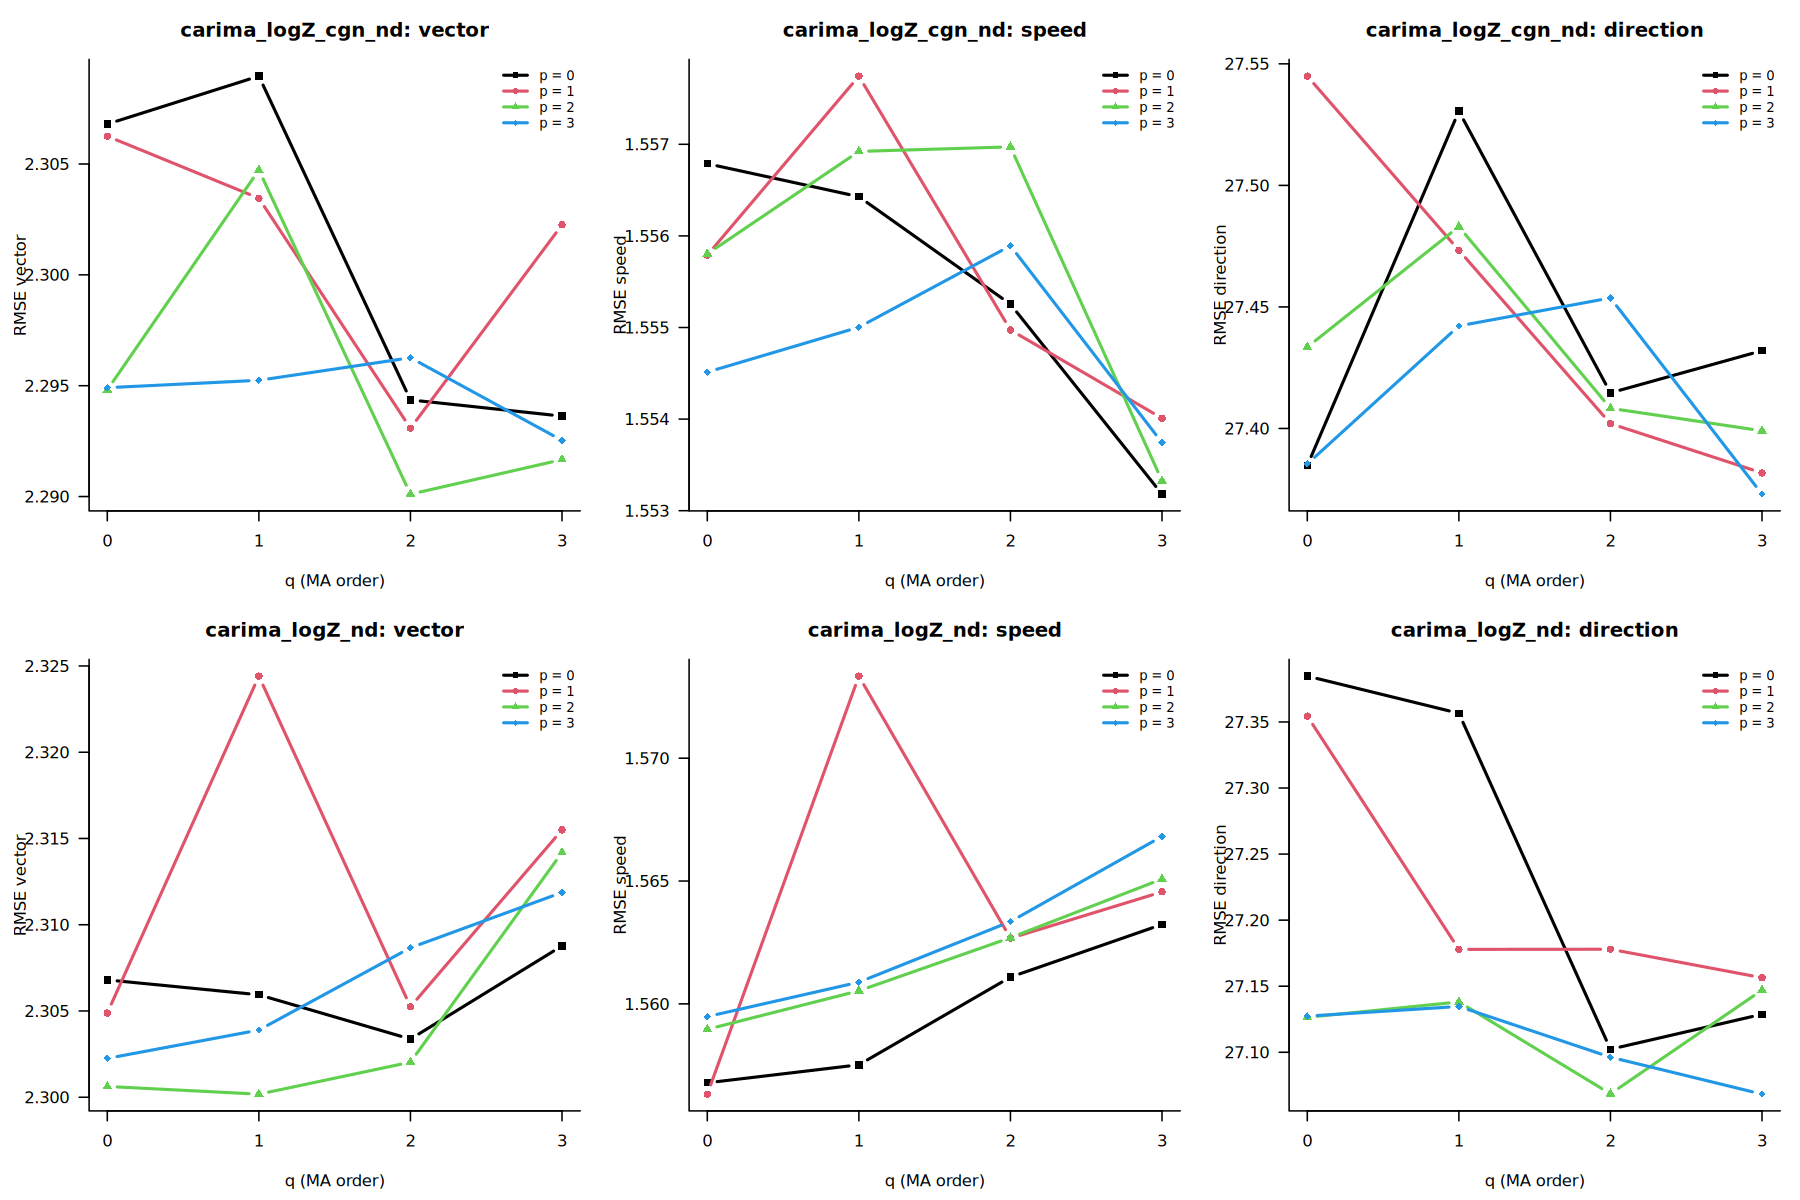
\includegraphics[width=\textwidth]{../figures/exp2_allorders_test.png}
  \caption{RMSE over the 300 test origins and $h = 1$--$12$ of all cARIMA$(p,1,q)$ for $\log Z$
    without a constant (top: generalised normal, bottom: normal), against $q$, one line for each
    $p$.}\label{fig:diag}
\end{figure}

\section{Accuracy of the point forecasts}\label{sec:accuracy}

Tables~\ref{tab:rmse-speed}--\ref{tab:rmse-z} give the RMSE over the 300 test origins at selected
horizons; all 12 horizons are in \code{results/exp2/tables/rmse\_\{speed,direction,vector\}.csv}.
Bold marks the lowest value in each column. All models produced forecasts at all origins. The
differences between models are small: the best model in each table is less than 1\% better than
persistence over all horizons.
\begin{itemize}
  \item \textbf{Speed.} At $h = 1$ and $h = 3$ the cARIMA models for $\log Z$ with the generalised
    normal error are best (0.705 and 1.044\,m/s against 0.710 and 1.048 for persistence), as in the
    first experiment. From $h = 6$ on, \code{arima\_speed\_angle}, which models speed directly, is
    best (1.545 over all horizons against 1.557). The models for $Z$ with $d = 0$
    (\code{auto\_carima\_z}, \code{auto\_carima\_z\_cgn}) are already worse than persistence at
    2 hours, because their forecasts move towards the short mean wind vector.
  \item \textbf{Direction.} The normal models for $\log Z$ without a rotating drift are best:
    \code{carima\_logZ\_re} ($27.10^\circ$) and \code{carima\_logZ\_nd} ($27.14^\circ$) against
    $27.38^\circ$ for persistence. The models with a rotating drift
    (\code{auto\_carima\_logZ} and the real pairs with the angle model) are the worst, but over 2
    hours the rotation has much less effect than over 6 hours.
  \item \textbf{Vector.} \code{auto\_carima\_z\_cgn} (2.291), \code{carima\_z\_cgn} (2.293) and the
    cARIMA models for $\log Z$ with the generalised normal error (2.294--2.300) are best, against
    2.307 for persistence; \code{carima\_logZ\_cgn\_nd} is best at $h = 1$. The real pairs with the
    angle model are 4--5\% worse than persistence.
\end{itemize}

\begin{table}[H]
  \centering
  \caption{RMSE of speed $|\hat Z|$ (m/s).}\label{tab:rmse-speed}
  \begin{tabular}{lrrrrr}
    \toprule
    model & $h=1$ & $h=3$ & $h=6$ & $h=12$ & $h=1$--$12$ \\
    \midrule
\texttt{persistence} & 0.710 & 1.048 & 1.571 & 1.995 & 1.557 \\ \midrule
\texttt{carima\_logZ} & 0.714 & 1.055 & 1.570 & 1.994 & 1.560 \\
\texttt{carima\_logZ\_cgn} & 0.707 & 1.046 & 1.577 & 2.014 & 1.565 \\
\texttt{carima\_logZ\_nd} & 0.713 & 1.054 & 1.571 & 1.994 & 1.560 \\
\texttt{carima\_logZ\_cgn\_nd} & 0.706 & 1.046 & 1.568 & 1.990 & 1.554 \\
\texttt{carima\_logZ\_re} & 0.713 & 1.059 & 1.575 & 2.001 & 1.565 \\
\texttt{carima\_logZ\_cgn\_re} & 0.706 & 1.050 & 1.574 & 2.005 & 1.563 \\
\texttt{carima\_z} & 0.716 & 1.054 & 1.569 & 1.990 & 1.556 \\
\texttt{carima\_z\_cgn} & 0.717 & 1.052 & 1.565 & 1.989 & 1.555 \\ \midrule
\texttt{auto\_carima\_logZ} & 0.711 & 1.058 & 1.571 & 1.980 & 1.558 \\
\texttt{auto\_carima\_logZ\_cgn} & \textbf{0.705} & \textbf{1.044} & 1.569 & 1.992 & 1.555 \\
\texttt{auto\_carima\_z} & 0.724 & 1.074 & 1.601 & 2.059 & 1.607 \\
\texttt{auto\_carima\_z\_cgn} & 0.721 & 1.066 & 1.589 & 2.042 & 1.591 \\ \midrule
\texttt{arima\_logSpeed\_angle} & 0.727 & 1.083 & 1.598 & 2.014 & 1.592 \\
\texttt{arima\_re\_im} & 0.727 & 1.054 & 1.569 & 1.978 & 1.557 \\
\texttt{arima\_speed\_angle} & 0.720 & 1.047 & \textbf{1.557} & \textbf{1.951} & \textbf{1.545} \\
\texttt{msarima\_logSpeed\_angle} & 0.731 & 1.089 & 1.609 & 2.019 & 1.598 \\
\texttt{msarima\_re\_im} & 0.728 & 1.061 & 1.573 & 1.996 & 1.563 \\
\texttt{msarima\_speed\_angle} & 0.718 & 1.052 & 1.571 & 1.972 & 1.558 \\
    \bottomrule
  \end{tabular}
\end{table}

\begin{table}[H]
  \centering
  \caption{RMSE of direction (degrees). The pairs \code{*\_speed\_angle} and
    \code{*\_logSpeed\_angle} use the same angle model and have identical rows.}\label{tab:rmse-angle}
  \begin{tabular}{lrrrrr}
    \toprule
    model & $h=1$ & $h=3$ & $h=6$ & $h=12$ & $h=1$--$12$ \\
    \midrule
\texttt{persistence} & 12.42 & 20.74 & 26.78 & 36.49 & 27.38 \\ \midrule
\texttt{carima\_logZ} & 12.66 & 20.72 & 26.72 & 36.96 & 27.53 \\
\texttt{carima\_logZ\_cgn} & 12.51 & 20.94 & 26.84 & 36.57 & 27.45 \\
\texttt{carima\_logZ\_nd} & 12.69 & 20.55 & 26.47 & 36.35 & 27.14 \\
\texttt{carima\_logZ\_cgn\_nd} & 12.47 & 20.83 & 26.77 & 36.53 & 27.39 \\
\texttt{carima\_logZ\_re} & 12.70 & \textbf{20.53} & \textbf{26.42} & 36.33 & \textbf{27.10} \\
\texttt{carima\_logZ\_cgn\_re} & 12.51 & 20.94 & 26.85 & 36.59 & 27.44 \\
\texttt{carima\_z} & 12.55 & 20.93 & 26.86 & 36.51 & 27.45 \\
\texttt{carima\_z\_cgn} & 12.73 & 20.96 & 26.98 & 36.34 & 27.45 \\ \midrule
\texttt{auto\_carima\_logZ} & 12.47 & 20.95 & 27.07 & 37.31 & 27.87 \\
\texttt{auto\_carima\_logZ\_cgn} & 12.48 & 20.85 & 26.80 & 36.54 & 27.41 \\
\texttt{auto\_carima\_z} & 12.94 & 21.43 & 27.48 & 36.41 & 27.70 \\
\texttt{auto\_carima\_z\_cgn} & 12.76 & 21.35 & 27.39 & \textbf{36.12} & 27.58 \\ \midrule
\texttt{arima\_logSpeed\_angle} & 12.49 & 21.09 & 27.15 & 37.27 & 27.88 \\
\texttt{arima\_re\_im} & 12.87 & 21.14 & 27.06 & 36.75 & 27.63 \\
\texttt{arima\_speed\_angle} & 12.49 & 21.09 & 27.15 & 37.27 & 27.88 \\
\texttt{msarima\_logSpeed\_angle} & \textbf{12.38} & 21.15 & 27.29 & 37.27 & 27.94 \\
\texttt{msarima\_re\_im} & 12.74 & 20.85 & 26.78 & 36.58 & 27.43 \\
\texttt{msarima\_speed\_angle} & \textbf{12.38} & 21.15 & 27.29 & 37.27 & 27.94 \\
    \bottomrule
  \end{tabular}
\end{table}

\begin{table}[H]
  \centering
  \caption{RMSE of the wind vector $|\hat Z - Z|$ (m/s).}\label{tab:rmse-z}
  \begin{tabular}{lrrrrr}
    \toprule
    model & $h=1$ & $h=3$ & $h=6$ & $h=12$ & $h=1$--$12$ \\
    \midrule
\texttt{persistence} & 0.960 & 1.634 & 2.307 & 2.996 & 2.307 \\ \midrule
\texttt{carima\_logZ} & 0.964 & 1.652 & 2.356 & 3.128 & 2.384 \\
\texttt{carima\_logZ\_cgn} & 0.954 & 1.619 & 2.300 & 2.994 & 2.300 \\
\texttt{carima\_logZ\_nd} & 0.961 & 1.627 & 2.294 & 2.989 & 2.300 \\
\texttt{carima\_logZ\_cgn\_nd} & \textbf{0.953} & 1.622 & 2.295 & 2.982 & 2.295 \\
\texttt{carima\_logZ\_re} & 0.962 & 1.633 & 2.298 & 2.998 & 2.307 \\
\texttt{carima\_logZ\_cgn\_re} & 0.955 & 1.625 & 2.297 & 2.986 & 2.298 \\
\texttt{carima\_z} & 0.964 & 1.639 & 2.314 & 2.994 & 2.311 \\
\texttt{carima\_z\_cgn} & 0.965 & 1.627 & 2.296 & 2.971 & 2.293 \\ \midrule
\texttt{auto\_carima\_logZ} & 0.960 & 1.657 & 2.355 & 3.110 & 2.379 \\
\texttt{auto\_carima\_logZ\_cgn} & 0.954 & \textbf{1.619} & 2.294 & 2.982 & 2.294 \\
\texttt{auto\_carima\_z} & 0.965 & 1.630 & 2.300 & 2.956 & 2.296 \\
\texttt{auto\_carima\_z\_cgn} & 0.964 & 1.636 & 2.301 & \textbf{2.951} & \textbf{2.291} \\ \midrule
\texttt{arima\_logSpeed\_angle} & 0.971 & 1.684 & 2.390 & 3.150 & 2.417 \\
\texttt{arima\_re\_im} & 0.974 & 1.631 & \textbf{2.294} & 2.969 & 2.298 \\
\texttt{arima\_speed\_angle} & 0.968 & 1.669 & 2.374 & 3.132 & 2.400 \\
\texttt{msarima\_logSpeed\_angle} & 0.975 & 1.696 & 2.411 & 3.165 & 2.432 \\
\texttt{msarima\_re\_im} & 0.973 & 1.645 & 2.309 & 2.996 & 2.312 \\
\texttt{msarima\_speed\_angle} & 0.967 & 1.676 & 2.383 & 3.143 & 2.408 \\
    \bottomrule
  \end{tabular}
\end{table}

\section{Accuracy of the predictive distributions}\label{sec:probabilistic}

\subsection{Pinball score}

Tables~\ref{tab:pinball-speed} and~\ref{tab:pinball-angle} give the pinball score averaged over
the 99 quantiles; the score for each $\tau$ is in
\code{results/exp2/tables/pinball\_by\_tau\_\{speed,direction\}.csv}, and Figure~\ref{fig:pinball}
plots the scores against the horizon.
\begin{itemize}
  \item \textbf{Direction: cARIMA for $Z$ is best.} \code{carima\_z\_cgn} has 5.53 over all
    horizons against 5.92 for persistence, 7\% better, and is best at every horizon except $h = 1$,
    where \code{auto\_carima\_z\_cgn} is best. The other models for $Z$ and the pairs of real models
    for $\Re Z$ and $\Im Z$ (5.58--5.62) follow. The generalised normal improves on the normal
    error for every series.
  \item \textbf{Speed: no clear winner.} \code{arima\_speed\_angle} (0.409), persistence (0.410),
    \code{arima\_re\_im} (0.411), \code{msarima\_speed\_angle} (0.412) and \code{carima\_z\_cgn}
    (0.412) are within 1\%. \code{carima\_z\_cgn} is best at $h = 1$--$3$ and $h = 5$,
    \code{arima\_speed\_angle} from $h = 7$ on.
  \item \textbf{The models for $\log Z$ have poor distributions} although their point forecasts are
    among the best. All cARIMA models for $\log Z$ are worse than persistence: by 13--14\% for
    speed and 6\% for direction with the generalised normal error, and by 21--24\% and 11--15\%
    with the normal error. The pairs of real models with log speed are 14\% worse for speed, and
    the pairs with the angle model are 16--17\% worse for direction.
\end{itemize}
The reason for the poor scores is the calibration, below: the point forecasts of these models are
as good as the others', so their quantiles must be too far from the actual values.

\begin{table}[H]
  \centering
  \caption{Pinball score of speed (m/s), averaged over $\tau = 0.01, \dots, 0.99$.}\label{tab:pinball-speed}
  \begin{tabular}{lrrrrr}
    \toprule
    model & $h=1$ & $h=3$ & $h=6$ & $h=12$ & $h=1$--$12$ \\
    \midrule
\texttt{persistence} & 0.1908 & 0.2880 & 0.4210 & 0.5474 & 0.4099 \\ \midrule
\texttt{carima\_logZ} & 0.2264 & 0.3595 & 0.5071 & 0.6763 & 0.4980 \\
\texttt{carima\_logZ\_cgn} & 0.1973 & 0.3205 & 0.4757 & 0.6454 & 0.4657 \\
\texttt{carima\_logZ\_nd} & 0.2261 & 0.3592 & 0.5085 & 0.6780 & 0.4991 \\
\texttt{carima\_logZ\_cgn\_nd} & 0.1971 & 0.3208 & 0.4751 & 0.6433 & 0.4650 \\
\texttt{carima\_logZ\_re} & 0.2261 & 0.3595 & 0.5082 & 0.6774 & 0.4989 \\
\texttt{carima\_logZ\_cgn\_re} & 0.1975 & 0.3216 & 0.4754 & 0.6434 & 0.4654 \\
\texttt{carima\_z} & 0.1924 & 0.2918 & 0.4263 & 0.5697 & 0.4194 \\
\texttt{carima\_z\_cgn} & \textbf{0.1908} & \textbf{0.2872} & 0.4191 & 0.5570 & 0.4123 \\ \midrule
\texttt{auto\_carima\_logZ} & 0.2255 & 0.3627 & 0.5169 & 0.6905 & 0.5066 \\
\texttt{auto\_carima\_logZ\_cgn} & 0.1967 & 0.3201 & 0.4750 & 0.6441 & 0.4651 \\
\texttt{auto\_carima\_z} & 0.1943 & 0.2928 & 0.4232 & 0.5516 & 0.4162 \\
\texttt{auto\_carima\_z\_cgn} & 0.1915 & 0.2896 & 0.4215 & 0.5538 & 0.4143 \\ \midrule
\texttt{arima\_logSpeed\_angle} & 0.2280 & 0.3514 & 0.4788 & 0.6067 & 0.4675 \\
\texttt{arima\_re\_im} & 0.1950 & 0.2894 & \textbf{0.4180} & 0.5473 & 0.4107 \\
\texttt{arima\_speed\_angle} & 0.1947 & 0.2898 & 0.4180 & \textbf{0.5383} & \textbf{0.4085} \\
\texttt{msarima\_logSpeed\_angle} & 0.2285 & 0.3517 & 0.4812 & 0.6069 & 0.4686 \\
\texttt{msarima\_re\_im} & 0.1950 & 0.2918 & 0.4235 & 0.5615 & 0.4166 \\
\texttt{msarima\_speed\_angle} & 0.1943 & 0.2915 & 0.4209 & 0.5444 & 0.4115 \\
    \bottomrule
  \end{tabular}
\end{table}

\begin{table}[H]
  \centering
  \caption{Pinball score of direction (degrees), averaged over $\tau = 0.01, \dots, 0.99$.}\label{tab:pinball-angle}
  \begin{tabular}{lrrrrr}
    \toprule
    model & $h=1$ & $h=3$ & $h=6$ & $h=12$ & $h=1$--$12$ \\
    \midrule
\texttt{persistence} & 2.493 & 4.429 & 5.906 & 8.487 & 5.917 \\ \midrule
\texttt{carima\_logZ} & 2.897 & 4.989 & 6.642 & 9.516 & 6.664 \\
\texttt{carima\_logZ\_cgn} & 2.511 & 4.607 & 6.297 & 9.070 & 6.273 \\
\texttt{carima\_logZ\_nd} & 2.903 & 4.956 & 6.588 & 9.349 & 6.590 \\
\texttt{carima\_logZ\_cgn\_nd} & 2.507 & 4.595 & 6.297 & 9.068 & 6.272 \\
\texttt{carima\_logZ\_re} & 2.905 & 4.952 & 6.571 & 9.336 & 6.580 \\
\texttt{carima\_logZ\_cgn\_re} & 2.519 & 4.609 & 6.295 & 9.072 & 6.275 \\
\texttt{carima\_z} & 2.341 & 4.159 & 5.623 & 7.946 & 5.582 \\
\texttt{carima\_z\_cgn} & 2.326 & \textbf{4.112} & \textbf{5.571} & \textbf{7.848} & \textbf{5.525} \\ \midrule
\texttt{auto\_carima\_logZ} & 2.885 & 5.046 & 6.762 & 9.689 & 6.775 \\
\texttt{auto\_carima\_logZ\_cgn} & 2.507 & 4.596 & 6.289 & 9.062 & 6.270 \\
\texttt{auto\_carima\_z} & 2.369 & 4.221 & 5.713 & 7.940 & 5.622 \\
\texttt{auto\_carima\_z\_cgn} & \textbf{2.318} & 4.161 & 5.659 & 7.857 & 5.570 \\ \midrule
\texttt{arima\_logSpeed\_angle} & 2.874 & 5.108 & 6.882 & 9.823 & 6.872 \\
\texttt{arima\_re\_im} & 2.386 & 4.209 & 5.633 & 7.942 & 5.610 \\
\texttt{arima\_speed\_angle} & 2.874 & 5.108 & 6.882 & 9.823 & 6.872 \\
\texttt{msarima\_logSpeed\_angle} & 2.866 & 5.130 & 6.961 & 9.910 & 6.929 \\
\texttt{msarima\_re\_im} & 2.369 & 4.170 & 5.609 & 7.946 & 5.585 \\
\texttt{msarima\_speed\_angle} & 2.866 & 5.130 & 6.961 & 9.910 & 6.929 \\
    \bottomrule
  \end{tabular}
\end{table}

\begin{figure}[H]
  \centering
  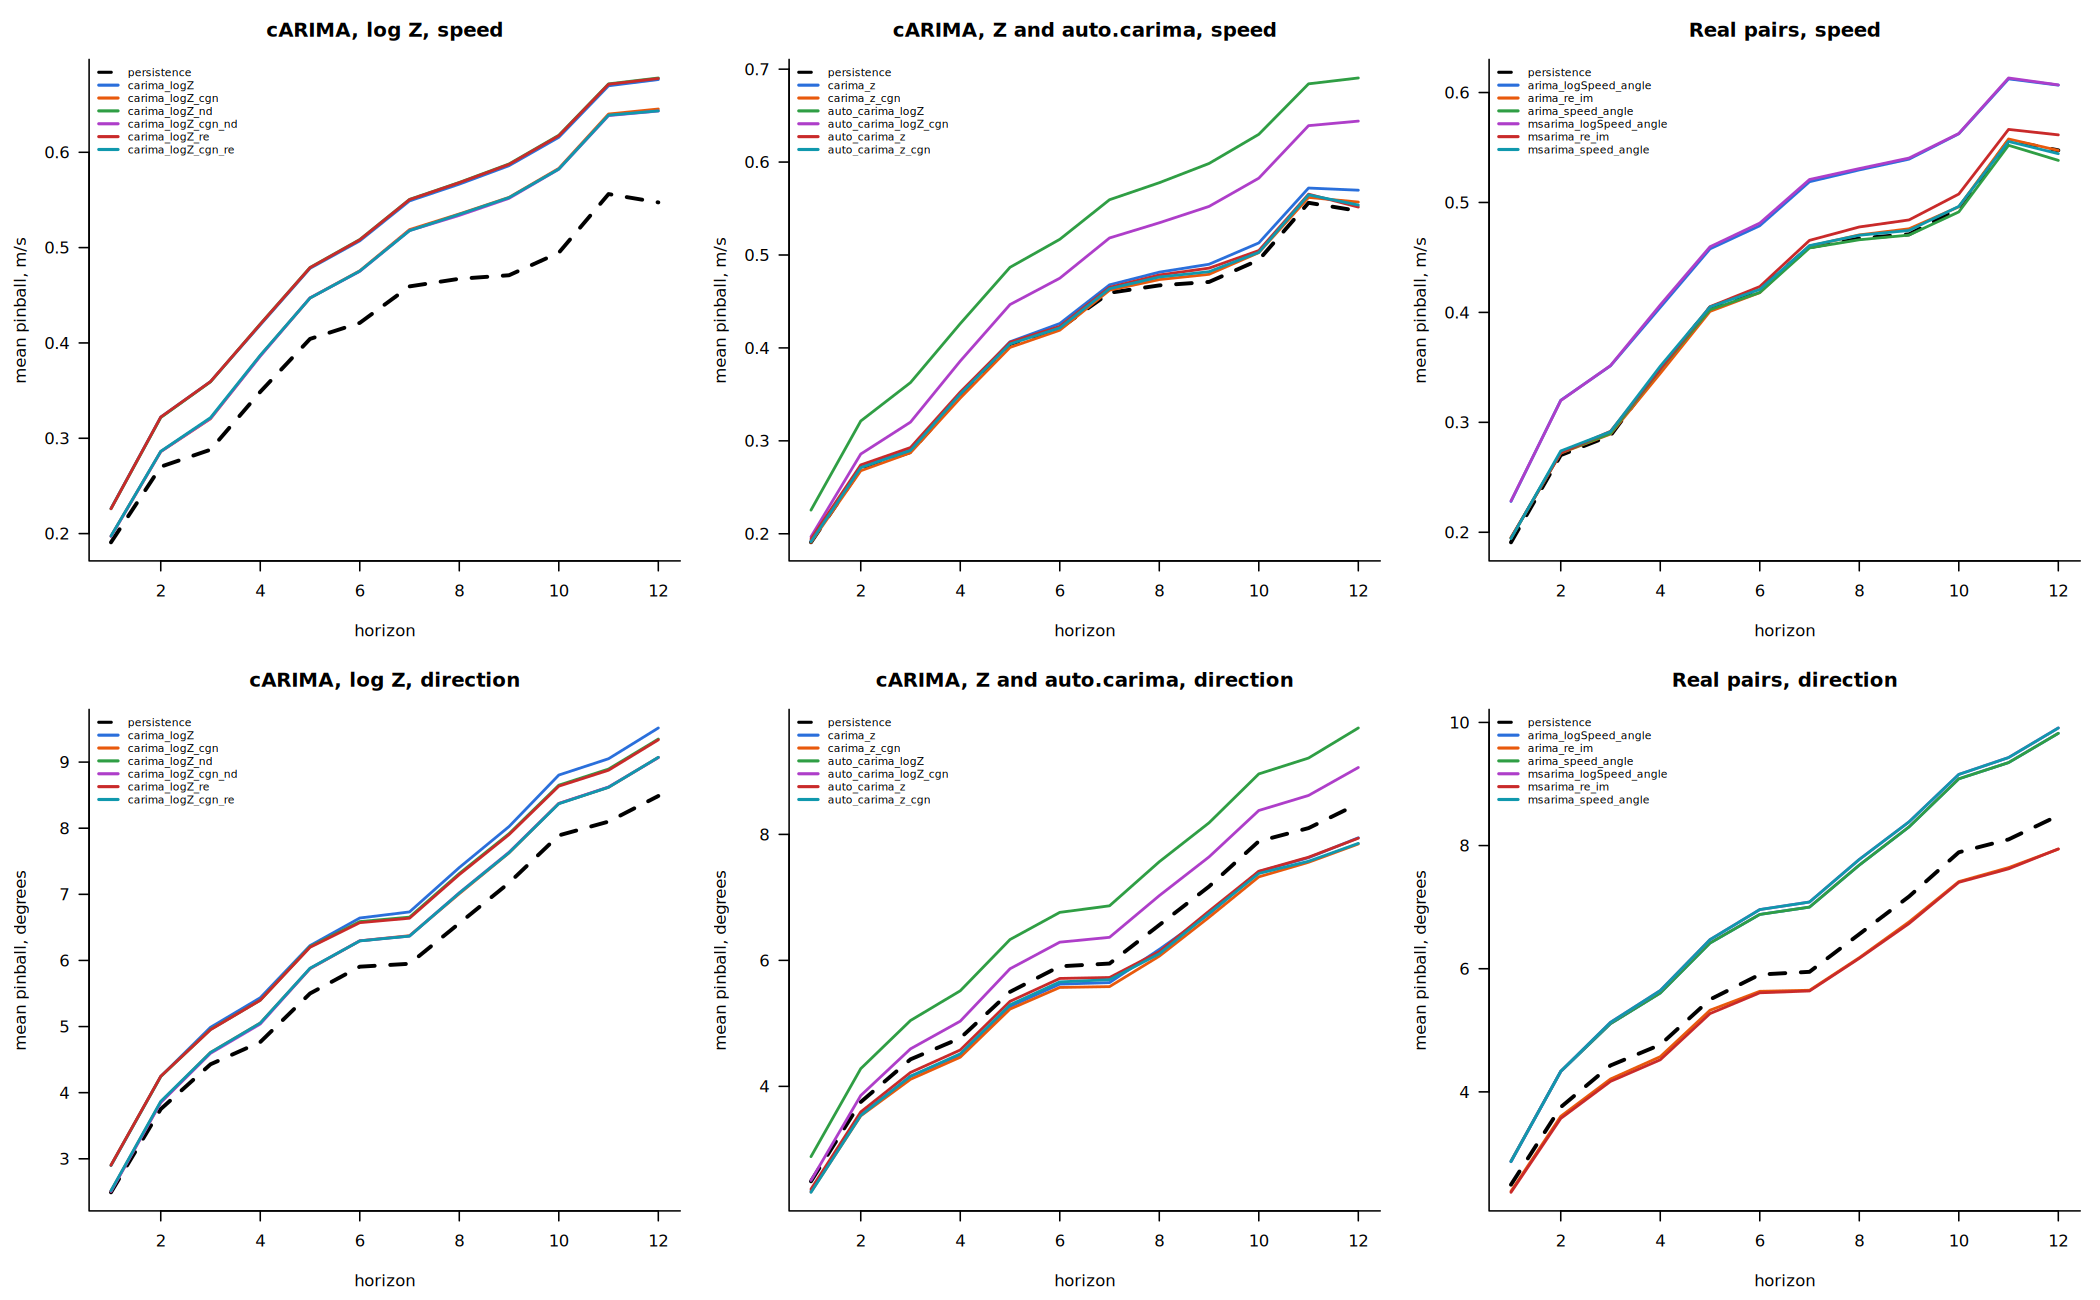
\includegraphics[width=\textwidth]{../figures/exp2_pinball.png}
  \caption{Pinball score averaged over $\tau$, against the horizon. Top: speed (m/s); bottom:
    direction (degrees). Persistence is the dashed black line in every panel.}\label{fig:pinball}
\end{figure}

\subsection{Calibration}

Figures~\ref{fig:calib-speed} and~\ref{fig:calib-angle} are the calibration plots, for the
average over $h = 1$--$12$ (top) and for $h = 1$ (bottom); Table~\ref{tab:calib} summarises them.
All values for $h = 1$--$12$, $h = 1$, $h = 6$ and $h = 12$ are in
\code{results/exp2/tables/calibration\_\{speed,direction\}.csv}.
\begin{itemize}
  \item \textbf{Persistence is well calibrated}, with a mean absolute calibration error of 0.014 for
    speed and 0.026 for direction, and central intervals that cover close to their nominal
    50\%, 80\% and 98\%. Its bootstrap reproduces the distribution of the $h$-step changes in the
    window.
  \item \textbf{Almost all models have intervals that are too wide in the centre.} The
    calibration curves are S-shaped: below $\tau = 0.5$ fewer actual values than nominal fall
    below the quantile, and above $\tau = 0.5$ more. So the quantiles near the median are too far
    from it. The 50\% intervals of the normal models for $\log Z$ cover 72--73\% of the actual
    speeds and 79--80\% of the directions; with the generalised normal error, 62--63\% and 72\%. In the tails it
    is the other way round: the 98\% intervals of most models cover only 96--98\%.
  \item \textbf{The best calibrated models} are \code{auto\_carima\_z\_cgn} for speed (0.015, as
    good as persistence) and \code{carima\_z\_cgn} for direction (0.022, better than persistence).
    For direction they are followed by the real pairs for $\Re Z$ and $\Im Z$ and the other models
    for $Z$ (0.028--0.038). The worst are
    the normal models for $\log Z$ and the real pairs with the angle model (0.11 for direction).
  \item \textbf{The generalised normal helps most at $h = 1$}: for the models for $\log Z$ it cuts
    the calibration error of direction from 0.12 to 0.03 at $h = 1$, but only from 0.10 to 0.085 at
    $h = 12$. The sum \eqref{eq:psi} of independent generalised normal innovations becomes closer
    to normal as $h$ grows, while the actual 2-hour changes remain sharply peaked.
\end{itemize}

\begin{table}[H]
  \centering
  \caption{Calibration over $h = 1$--$12$: mean absolute calibration error over $\tau$ (MACE) and
    coverage of the central 50\%, 80\% and 98\% intervals.}\label{tab:calib}
  \resizebox{\textwidth}{!}{%
  \begin{tabular}{lrrrrrrrr}
    \toprule
    & \multicolumn{4}{c}{speed} & \multicolumn{4}{c}{direction} \\
    \cmidrule(lr){2-5}\cmidrule(lr){6-9}
    model & MACE & 50\% & 80\% & 98\% & MACE & 50\% & 80\% & 98\% \\
    \midrule
\texttt{persistence} & \textbf{0.014} & 0.501 & 0.789 & 0.978 & 0.026 & 0.497 & 0.794 & 0.977 \\ \midrule
\texttt{carima\_logZ} & 0.074 & 0.722 & 0.889 & 0.974 & 0.108 & 0.794 & 0.911 & 0.968 \\
\texttt{carima\_logZ\_cgn} & 0.041 & 0.624 & 0.847 & 0.979 & 0.077 & 0.718 & 0.890 & 0.971 \\
\texttt{carima\_logZ\_nd} & 0.075 & 0.724 & 0.890 & 0.976 & 0.107 & 0.799 & 0.913 & 0.969 \\
\texttt{carima\_logZ\_cgn\_nd} & 0.042 & 0.627 & 0.849 & 0.979 & 0.076 & 0.716 & 0.888 & 0.972 \\
\texttt{carima\_logZ\_re} & 0.074 & 0.723 & 0.889 & 0.975 & 0.106 & 0.799 & 0.912 & 0.968 \\
\texttt{carima\_logZ\_cgn\_re} & 0.041 & 0.620 & 0.849 & 0.979 & 0.076 & 0.716 & 0.888 & 0.971 \\
\texttt{carima\_z} & 0.048 & 0.592 & 0.852 & 0.971 & 0.037 & 0.605 & 0.859 & 0.967 \\
\texttt{carima\_z\_cgn} & 0.036 & 0.556 & 0.831 & 0.972 & \textbf{0.022} & 0.556 & 0.831 & 0.967 \\ \midrule
\texttt{auto\_carima\_logZ} & 0.077 & 0.731 & 0.891 & 0.977 & 0.109 & 0.797 & 0.912 & 0.969 \\
\texttt{auto\_carima\_logZ\_cgn} & 0.041 & 0.626 & 0.847 & 0.981 & 0.076 & 0.716 & 0.889 & 0.971 \\
\texttt{auto\_carima\_z} & 0.024 & 0.580 & 0.832 & 0.967 & 0.038 & 0.599 & 0.852 & 0.968 \\
\texttt{auto\_carima\_z\_cgn} & 0.015 & 0.551 & 0.821 & 0.974 & 0.028 & 0.568 & 0.841 & 0.968 \\ \midrule
\texttt{arima\_logSpeed\_angle} & 0.053 & 0.652 & 0.852 & 0.963 & 0.114 & 0.809 & 0.916 & 0.972 \\
\texttt{arima\_re\_im} & 0.036 & 0.576 & 0.837 & 0.965 & 0.031 & 0.587 & 0.841 & 0.966 \\
\texttt{arima\_speed\_angle} & 0.026 & 0.579 & 0.831 & 0.965 & 0.114 & 0.809 & 0.916 & 0.972 \\
\texttt{msarima\_logSpeed\_angle} & 0.052 & 0.654 & 0.853 & 0.962 & 0.116 & 0.815 & 0.917 & 0.972 \\
\texttt{msarima\_re\_im} & 0.043 & 0.582 & 0.841 & 0.968 & 0.037 & 0.603 & 0.853 & 0.965 \\
\texttt{msarima\_speed\_angle} & 0.027 & 0.582 & 0.836 & 0.963 & 0.116 & 0.815 & 0.917 & 0.972 \\
    \bottomrule
  \end{tabular}}
\end{table}

\begin{figure}[H]
  \centering
  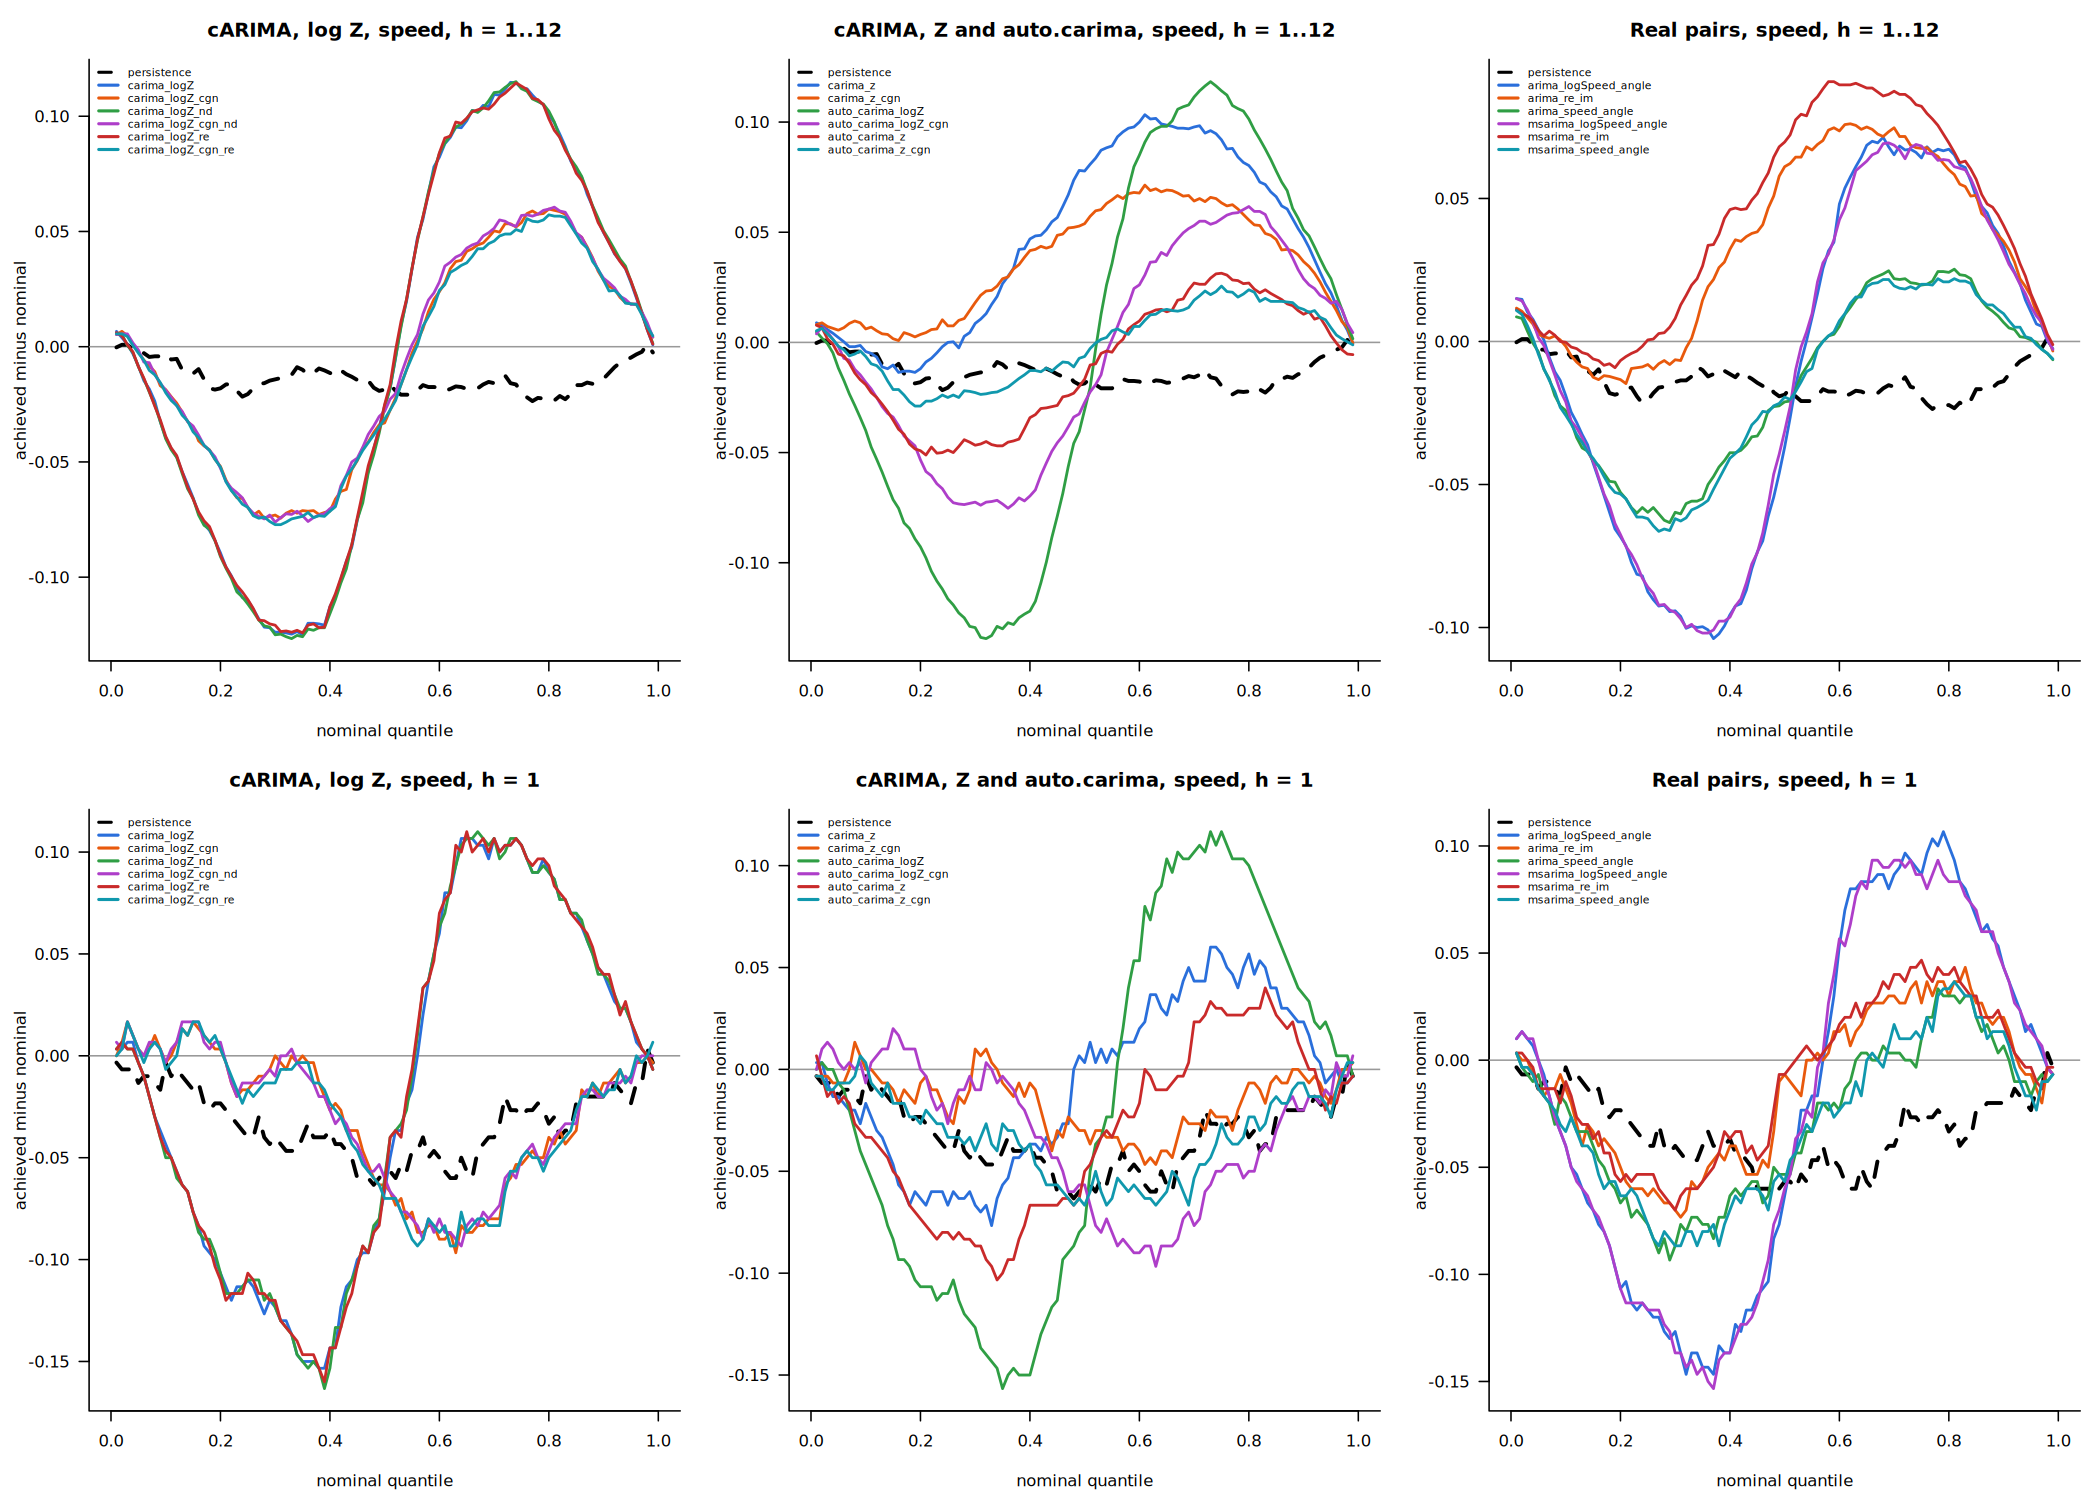
\includegraphics[width=\textwidth]{../figures/exp2_calibration_speed.png}
  \caption{Calibration of speed: share of actual values below the forecast $\tau$-quantile minus
    $\tau$, against $\tau$. Top: average over $h = 1$--$12$; bottom: $h = 1$. Persistence is the
    dashed black line in every panel.}\label{fig:calib-speed}
\end{figure}

\begin{figure}[H]
  \centering
  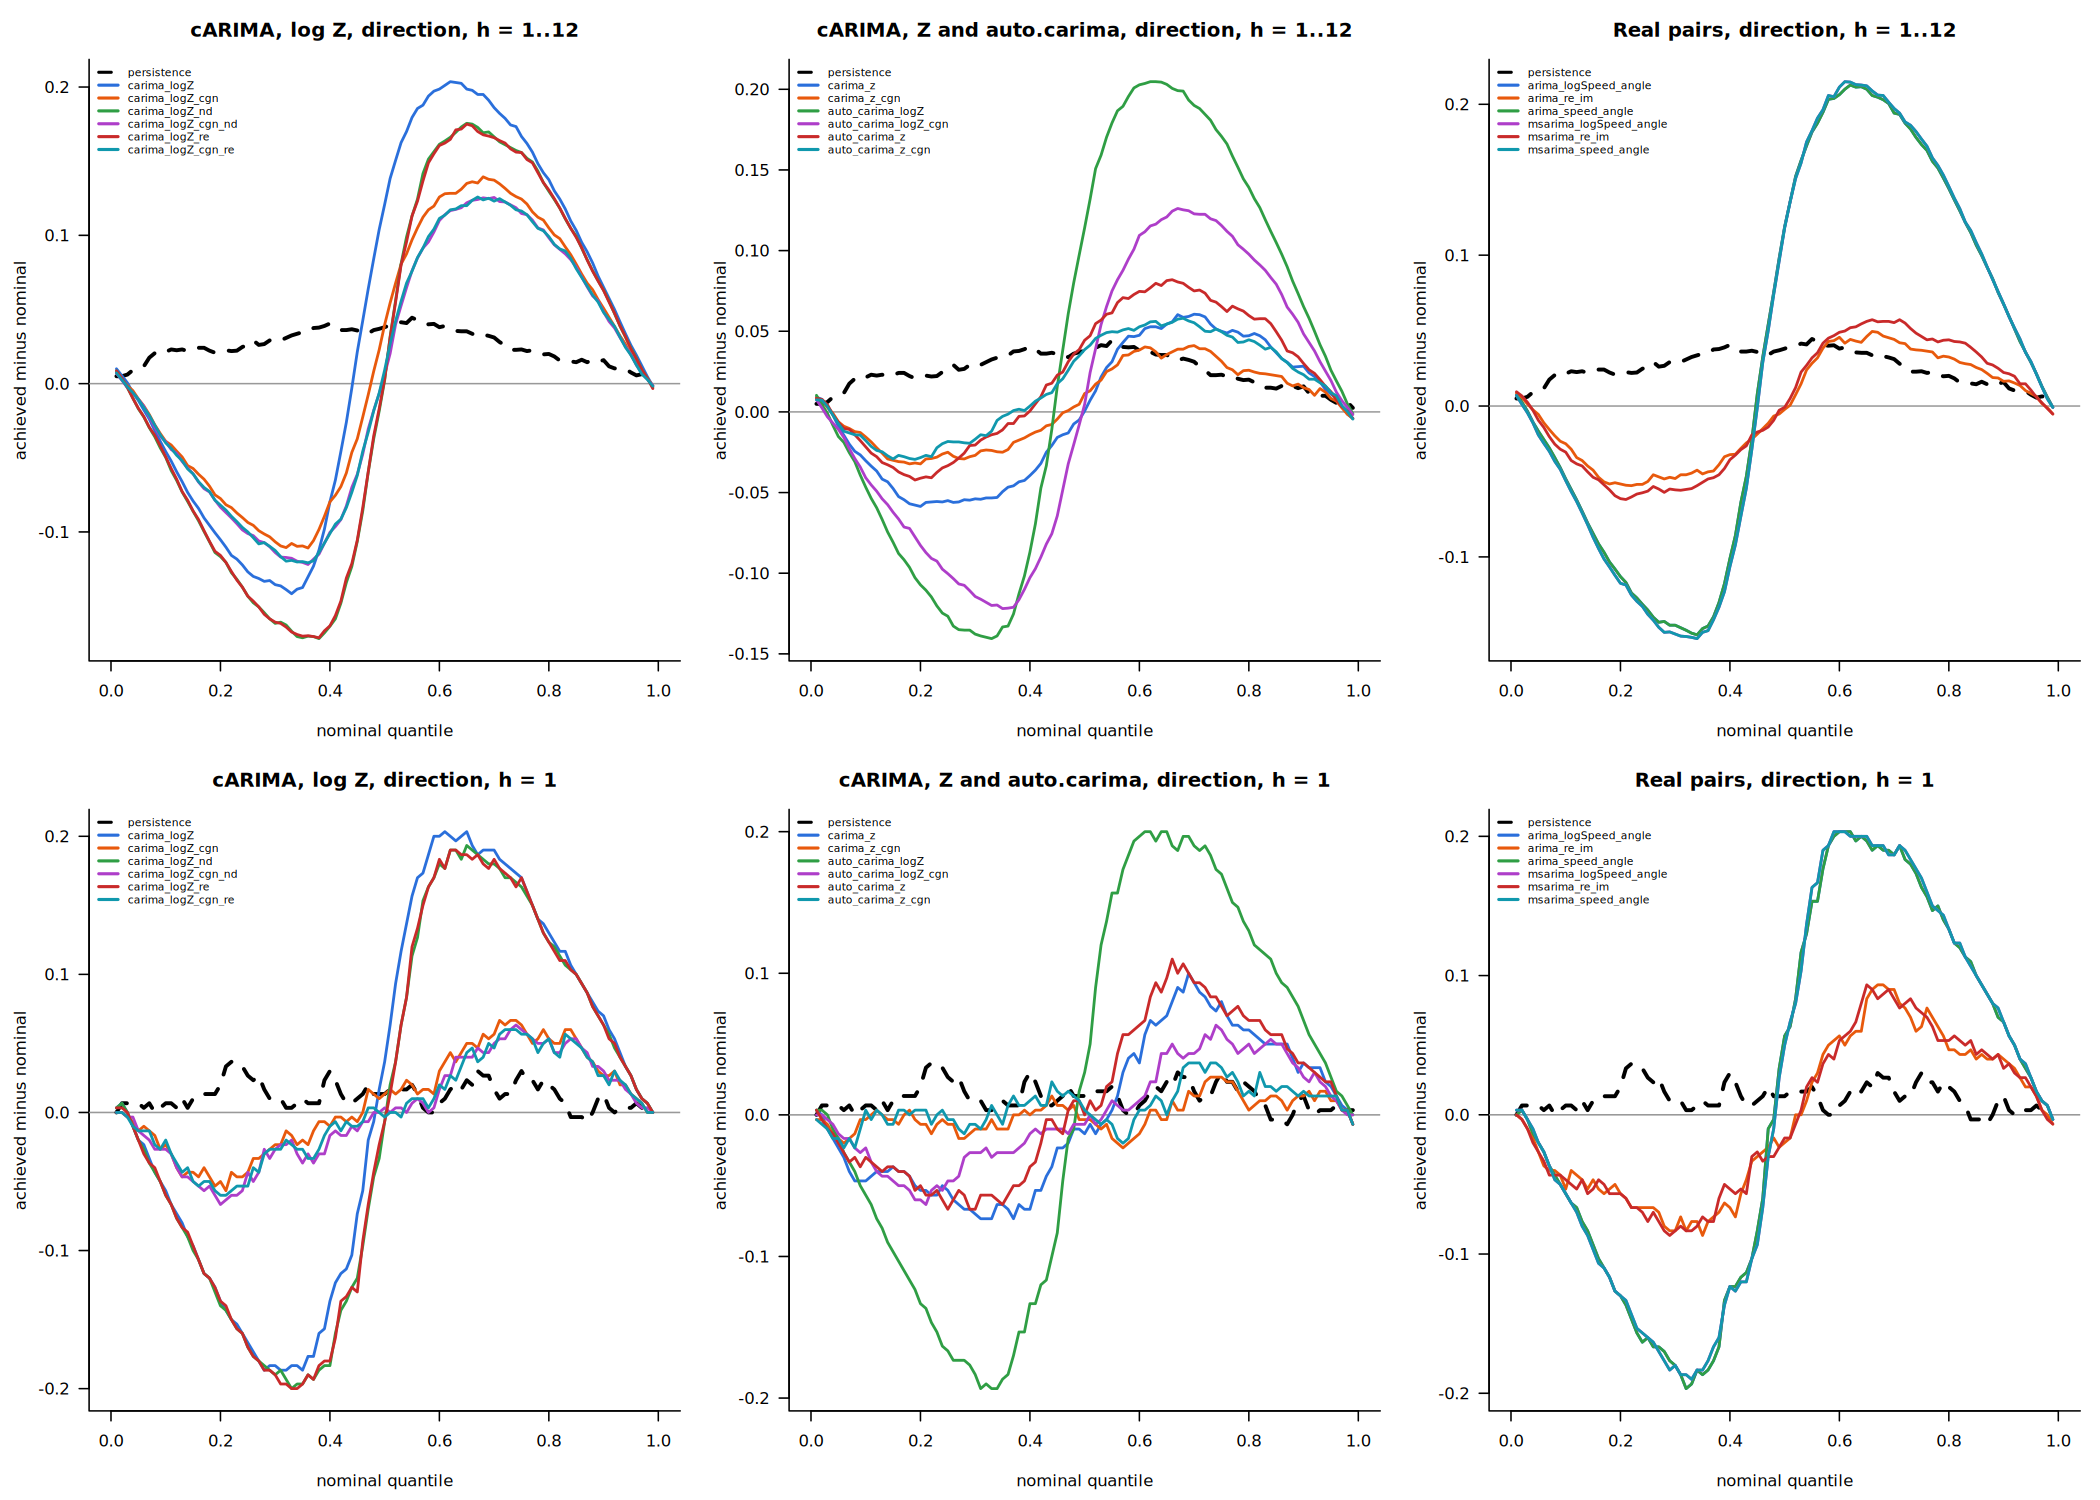
\includegraphics[width=\textwidth]{../figures/exp2_calibration_direction.png}
  \caption{Calibration of direction, as in Figure~\ref{fig:calib-speed}.}\label{fig:calib-angle}
\end{figure}

\section{Findings}

\begin{enumerate}
  \item \textbf{The cAR(0) orders were not a real feature of the data.} Cross-validation chooses
    $p > 0$ for 7 of 8 variants, but all orders forecast almost equally well (within 1\%), on the
    cross-validation and on the test origins. The AR and MA terms nearly cancel, so the orders are
    weakly identified, and whether the chosen model has $p = 0$ depends on the window and on the
    optimiser. The order does not matter for forecasting up to 2 hours.
  \item \textbf{Point forecasts up to 2 hours}: no model is more than 1\% better than persistence
    over all horizons. The best are \code{auto\_carima\_z\_cgn} and \code{carima\_z\_cgn} for the
    vector, \code{carima\_logZ\_re} and \code{carima\_logZ\_nd} for direction, and
    \code{arima\_speed\_angle} for speed; the cARIMA models for $\log Z$ with the generalised normal
    error are best at 10 and 30 minutes for speed and the vector.
  \item \textbf{The real constant} (comment 4) gives the best direction forecasts of all models
    ($27.10^\circ$), slightly ahead of no constant ($27.14^\circ$); for the vector and speed it is
    about equal to persistence.
  \item \textbf{Predictive distributions of direction: cARIMA for $Z$ with the generalised normal
    error is the best model} (pinball 7\% better than persistence, and better calibrated). It is
    also better than the two independent real models for $\Re Z$ and $\Im Z$, which ignore the
    correlation between the two errors.
  \item \textbf{Predictive distributions of speed}: persistence, the real model for speed and
    cARIMA for $Z$ with the generalised normal error are equally good.
  \item \textbf{The models for $\log Z$ give good point forecasts but poor distributions}: their
    intervals are much too wide in the centre. Changes of direction are large at low speeds and
    small at high speeds: the median 10-minute change is $11.0^\circ$ at speeds up to 3\,m/s,
    $2.6^\circ$ at 5--8\,m/s and $1.5^\circ$ above 12\,m/s. A model for $\log Z$ has one variance for
    the direction at all speeds, so at the usual speeds its direction intervals are too wide. In a
    model for $Z$, the same error of the wind vector is a large change of direction at low speed and
    a small one at high speed, as in the data.
  \item \textbf{The generalised normal error improves all distributions}, most at short
    horizons. For all models, the central intervals are still too wide and the extreme ones
    slightly too narrow, because the actual changes over 2 hours are more sharply peaked than the
    sums of independent innovations the models assume. Only the bootstrap of persistence, which uses
    the empirical $h$-step changes directly, is close to perfectly calibrated.
\end{enumerate}

\section{Limitations and next steps}

\begin{itemize}
  \item One turbine and one year; no tests of the differences in accuracy (e.g.\
    Diebold--Mariano); parameter uncertainty is ignored in the intervals.
  \item The explanation in finding 6 is not tested: the calibration could be computed separately
    for low and high speeds at the origin.
  \item The changes of wind are probably heteroscedastic (calm and turbulent periods), which would
    also explain why the actual 2-hour changes are more peaked than the model distributions. A
    model for the scale, or empirical intervals from the in-sample $h$-step errors of cARIMA (the
    \code{"empirical"} interval of \code{smooth}, not yet implemented in \code{complex}), may give
    better calibrated cARIMA distributions.
  \item The CRPS and an energy score for the joint distribution of speed and direction would
    evaluate the bivariate forecast directly, which is where a complex model should have an
    advantage.
  \item Not yet included: daily cycles (e.g.\ Fourier terms), VAR and VARMA benchmarks, forecasts
    of turbine power, and other datasets.
\end{itemize}

\section{Reproducing the results}\label{sec:reproduce}

\begin{verbatim}
Rscript R/02_prepare_data.R     # needs data/raw/T1.csv
Rscript R/08_phase_plane.R
Rscript R/09_exp2_origins.R     # test and cross-validation origins
results/exp2/run_orders.sh      # R/10_all_orders.R (cv, test), R/11
results/exp2/run_forecasts.sh   # installs complex, R/12, R/13
\end{verbatim}

\noindent Shared code is in \code{R/functions.R} and \code{R/exp2\_functions.R}. The orders of the
\code{auto\_carima} models and of the real benchmarks are read from
\code{results/tables/orders.csv} (first experiment). The \code{complex} package is the development
version with the prediction intervals (branch \code{intervals}). On 32 cores with 30 workers,
the cross-validation took 5.1 hours, the diagnostic on the test origins 3.0 hours, and the final
forecasts of the 19 models 1.6 hours.

\begin{thebibliography}{9}
\bibitem[Novey et~al.(2010)]{novey2010}
Novey, M., Adali, T. and Roy, A. (2010). A complex generalized Gaussian distribution:
characterization, generation, and estimation. \emph{IEEE Transactions on Signal Processing},
58(3), 1427--1433.
\bibitem[Svetunkov and Svetunkov(2024)]{svetunkov2024}
Svetunkov, S. and Svetunkov, I. (2024). \emph{Complex-Valued Econometrics with Examples in R}.
Springer.
\end{thebibliography}

\end{document}
